%% Paper v2: The Tax Base Decides
%% Compile from writing/: python3 make_paper_bib.py; pdflatex paper_v2; bibtex paper_v2; pdflatex paper_v2; pdflatex paper_v2
%% All numbers come from the v2.0-empirical-freeze outputs in generated/.

\documentclass[11pt,a4paper]{article}

\usepackage[utf8]{inputenc}
\usepackage[T1]{fontenc}
\usepackage{textcomp}
\usepackage{lmodern}
\usepackage[british]{babel}

\usepackage[a4paper, top=2.3cm, bottom=2.3cm, left=2.5cm, right=2.5cm]{geometry}

\usepackage{microtype}
\usepackage{setspace}
\onehalfspacing
\raggedbottom
\setlength{\parindent}{0pt}
\setlength{\parskip}{0.6em}
\setlength{\emergencystretch}{1.5em}

\usepackage{amsmath,amssymb}
\usepackage{booktabs}
\usepackage{longtable}
\usepackage{tabularx}
\usepackage{array}
\usepackage{graphicx}
\usepackage{float}
\usepackage{xcolor}
\usepackage{tikz}
\usetikzlibrary{arrows.meta, positioning}
\usepackage[font=small, labelfont=bf, skip=4pt]{caption}

\usepackage[round,authoryear]{natbib}
\setlength{\bibsep}{0.35\baselineskip}
\renewcommand{\bibfont}{\raggedright}

\usepackage[
  colorlinks = true,
  linkcolor  = blue!60!black,
  citecolor  = blue!60!black,
  urlcolor   = blue!60!black,
  pdftitle   = {The Tax Base Decides: Why Global Minimum Tax Revenue Estimates Disagree},
  pdfauthor  = {Maurits de Haan and Peter Gerbrands},
]{hyperref}

\usepackage{fancyhdr}
\pagestyle{fancy}
\fancyhf{}
\setlength{\headheight}{14pt}
\fancyhead[L]{\small\itshape\nouppercase{\leftmark}}
\fancyhead[R]{\small\itshape de Haan and Gerbrands (2026)}
\fancyfoot[C]{\small\thepage}
\renewcommand{\headrulewidth}{0.4pt}
\renewcommand{\sectionmark}[1]{\markboth{\thesection\quad #1}{}}
\fancypagestyle{plain}{\fancyhf{}\fancyfoot[C]{\small\thepage}\renewcommand{\headrulewidth}{0pt}}

\usepackage{titlesec}
\titleformat{\section}{\Large\bfseries\raggedright}{\thesection}{1em}{}
\titleformat{\subsection}{\large\bfseries\raggedright}{\thesubsection}{1em}{}
\titlespacing*{\section}{0pt}{12pt plus 2pt minus 2pt}{4pt plus 1pt minus 1pt}
\titlespacing*{\subsection}{0pt}{8pt plus 2pt minus 2pt}{2pt plus 1pt minus 1pt}

\newcommand{\EUR}{\texteuro}
\newcommand{\usd}{US\$}
\newcommand{\draftstub}[1]{\textit{[To be drafted in #1.]}}

\begin{document}

\thispagestyle{plain}
\begin{center}
  {\LARGE\bfseries The Tax Base Decides:\\[0.2em] Why Global Minimum Tax\\[0.1em] Revenue Estimates Disagree%
  \footnote{Working titles under discussion among the authors: \emph{Measurement before Behaviour: Decomposing Uncertainty in Europe's Global Minimum Tax Revenue} and \emph{Who Collects the Minimum Tax? Measurement, Accounting and Allocation in Public Country-by-Country Data}. The paper builds on the first author's MSc thesis at Utrecht University School of Economics. All data are public. The replication package, with pinned input extracts, code and a map from every exhibit to its inputs, is described in \texttt{REPLICATION.md}.}}\\[1.2em]
  {\large Maurits de Haan \qquad Peter Gerbrands}\\[0.3em]
  % Placeholder: Javier Garcia-Bernardo (Utrecht University, Methodology and Statistics), pending discussion.
  {\small Utrecht University School of Economics}\\[0.3em]
  {\small Draft, November 2026}
\end{center}

\begin{abstract}
\noindent European governments have budgeted revenue from the Global Minimum Tax, yet published estimates for the same country differ by multiples. We trace that disagreement to its sources. Using public OECD country-by-country data for 2017–2023, we compute European revenue under every combination of six modelling decisions and attribute the variance across estimates to each decision. Two decisions dominate: how profit taxed below 15\% is measured and how accounting profit is translated into the minimum-tax base. Together they explain 84.7–91.8\% of the variance. Statistical uncertainty in estimated parameters accounts for 1.71\% or less, and profit-shifting responses shrink once a division bias in effective tax rates is removed. After the accounting adjustments, the model tracks national budget forecasts for real-economy collectors. Under the 2026 Side-by-Side package, repealing a domestic top-up tax becomes a tax cut for US-parented groups: 85.9\% of Ireland's forgone revenue reaches firms.

\medskip
\noindent\textbf{JEL codes:} H25, H87, F23, C54\\
\textbf{Keywords:} global minimum tax; Pillar Two; country-by-country reporting; revenue estimation; profit shifting; tax competition
\end{abstract}

%% ===
\section{Introduction}\label{sec:introduction}

European governments have already written revenue from the new global minimum tax on multinational profits into their budgets, yet nobody can tell them which part of that forecast is solid. The Global Minimum Tax (GMT), agreed in October 2021 by 137 jurisdictions under the Inclusive Framework of the Organisation for Economic Co-operation and Development (OECD), sets a floor of 15\% on the effective tax rate (ETR) of multinational enterprises (MNEs) with consolidated revenue above \EUR750 million. Where the ETR in a country falls below the floor, a top-up tax closes the gap. The reform targets four decades of profit shifting, whose scale is itself estimated at \usd300–850 billion a year \citep{torslov2023,garcia-bernardo2024}. Member States of the European Union have applied the rules since fiscal year 2024 and count on the proceeds. The Dutch case shows how fragile the resulting forecasts are. The government first projected \EUR466 million a year, 86\% of it from reduced profit shifting \citep{36369_3}, and then lowered the projection by \EUR122 million when the January 2026 Side-by-Side package changed a single allocation rule \citep{1028}. Published academic estimates for the same country differ by multiples, and a finance ministry that compares them cannot see why.

Every revenue estimate rests on a short list of modelling decisions, and the size of the estimate depends on how each one is made. An analyst has to decide which profit counts as taxed below 15\%, how much of that profit the rules exempt because it reflects real activity, which exemption rates apply, how firms relocate profit once the floor binds, which government collects the tax, and how the accounting profit in the data maps into the legal tax base. We treat these six decisions as switches. By switching each decision on or off and computing revenue for the 27 Member States of the European Union (EU27) under every combination, we measure how much each decision moves the answer. The variance across the resulting scenarios is then attributed to main effects and interactions with a factorial design, in the spirit of Oaxaca–Blinder decompositions and Shapley attribution \citep{oaxaca1973,blinder1973,shorrocks2013}. The data are the public Country-by-Country Reporting (CbCR) statistics of the OECD for 2017–2023, which cover the last fiscal year before the tax took effect in the European Union.

Two of the six decisions account for almost all of the disagreement between estimates. In the 64-scenario design, the way effective tax rates are aggregated carries a Shapley share of 42.5–50.2\% of the variance in EU27 revenue, and the translation of accounting profit into the minimum-tax base carries 39.7–44.7\%. Jointly they explain 84.7–91.8\% across the 2017–2023 and 2019–2023 windows, and more than 93\% in 2021–2023, the window in which direct bracket data carry most of the measurement. The allocation regime, the substance exemption and the behavioural response share the remainder. The spread is large in absolute terms: across the 32 scenarios without the accounting decision, cumulative EU27 revenue over 2017–2023 ranges from \usd144.3 billion to \usd584.9 billion. Statistical uncertainty in the estimated parameters is negligible by comparison. It accounts for 1.71\% of total variance over 2017–2023 and 0.36\% over 2019–2023. Disagreement about revenue is therefore disagreement about the tax base. For a finance ministry the implication is practical: agreeing on how low-taxed profit is measured and how accounts map into the legal base narrows the range of defensible forecasts far more than refining the assumed behavioural response.

Three further results show that the ranking survives the most obvious objections to the method. The first concerns measurement. Fitting a distribution to published ETR percentiles overstates low-taxed profit in large domestic cells when the upper percentile exceeds 100\%; capping the percentiles at the statutory rate halves the validation error against directly observed data, from 3.85 to 1.74 percentage points. The second concerns behaviour. The steep profit-shifting responses that logarithmic specifications produce at low tax rates (semi-elasticities of 9.33–11.20 at an ETR of 5\%) largely reflect a division bias, because profit appears in the denominator of the ETR. Lagged and leave-one-parent-out tax rates reduce them to 2.51–3.94. The third concerns external validity. After the accounting adjustments, modelled 2023 revenue for Germany, France, Belgium, Austria, Slovakia and Ireland lies within \EUR0.5 billion of the figure in each national budget.

The decisions that matter for the total also decide which treasuries receive the money. Five Member States collect nothing in the preferred scenario, yet profit booked in them generates \usd11.94 billion of top-up tax over 2017–2023 that is collected abroad or extinguished by the Side-by-Side package. That package also changes the incentive to keep a domestic top-up tax. Under the original rules a state that repeals its tax hands the revenue to other governments, and multinationals gain nothing. Under Side-by-Side, repeal becomes a tax cut for groups parented in the United States: in Ireland 85.9\% of the forgone revenue reaches firms. A capped incentive tied to payroll and tangible assets, which the rules also permit, delivers relief in all 27 states without any revenue flowing abroad. Behaviour has a distributional counterpart as well. Profit that leaves low-tax countries lowers direct EU27 top-up tax by \usd58.1 billion over 2017–2023 and raises ordinary corporate tax where it lands by \usd65.3 billion before source-country losses, so a forecast that counts only the lost top-up tax misstates the fiscal effect of behaviour.

Earlier studies each fix most of these decisions and vary one, so their estimates cannot be compared. \citet{barake2022} provide the first global revenue estimate from CbCR data, but they use jurisdiction-average ETRs, which treat all profit in a country as lying on one side of the floor. \citet{hugger2026} show with confidential data that more than half of low-taxed profit sits in countries whose average ETR exceeds 15\%; their data cannot be accessed by other researchers, and they stop short of revenue by collecting state. We deliver a distributional measure from public data and validate it against direct observations. \citet{godar2024} and \citet{tuinsma2025} document what country-by-country reports reveal and where they mislead, without carrying those limits through to a revenue estimate. We carry them through by correcting double-counted profit and by testing the fitted distributions against bracket data. \citet{devereux2023} quantify the substance carve-out and \citet{schjelderup2024} analyse its incentive effects, each holding measurement fixed. We vary the carve-out jointly with measurement and find its contribution small once the base is measured distributionally. \citet{hanlon2023} explains why accounting profit departs from the legal tax base but offers no quantification, which our accounting bridge supplies. The behavioural literature ranges from a consensus semi-elasticity of 0.8 \citep{heckemeyer2017} to far steeper responses at low rates \citep{dowd2017,garcia-bernardo2024}, and none of these studies separates the response from the division bias that we correct. \citet{boukal2026} come closest to our design by decomposing revenue for Slovakia into top-up tax and reduced shifting; their decomposition covers one country and two channels. Ours covers 27 states and six decisions, and it attributes the interactions between them. Finally, \citet{devereux2022} and \citet{jean2026} analyse adoption and enforcement incentives in theory, which we test on all Member States under the 2026 rules. Four elements are introduced in this paper: the six-factor design that includes the accounting bridge, a four-level ladder of ETR aggregation, a ratio $\Lambda$ that compares scenario disagreement with parameter uncertainty, and a ledger that sets the liability each state generates against the revenue it collects.

The paper follows multinational profit from the public reports to the treasury that collects the tax. Section \ref{sec:institutions} sets out how the minimum tax turns low-taxed profit into revenue and which modelling decisions that process requires. Section \ref{sec:data} describes the data. Section \ref{sec:measurement} measures each filter, Section \ref{sec:decomposition} decomposes the disagreement between scenarios, Section \ref{sec:allocation} turns to collectors and their incentives, and Section \ref{sec:conclusion} concludes.

%% ===
\section{How the minimum tax raises revenue}\label{sec:institutions}

This section explains how the minimum tax converts profit into revenue, because every modelling decision studied later corresponds to one step in that conversion. Section \ref{sec:rules} describes the rules, Section \ref{sec:filters} writes revenue as a sequence of filters, and Section \ref{sec:disagree} shows where published estimates part ways.

\subsection{The collection rules}\label{sec:rules}

The minimum tax adds a top-up charge wherever a multinational pays less than fifteen per cent, and a fixed order of rules decides which government collects it. The order matters because the country where low-taxed profit is booked, the country where the group is headquartered and the other countries where the group operates all have a claim, and only one of them can be first. The model rules of the OECD give the host country the first claim through a qualified domestic minimum top-up tax (QDMTT). If the host does not levy one, the parent country collects through the income inclusion rule (IIR). If neither applies, other countries in which the group operates collect through the undertaxed profits rule (UTPR), a backstop \citep{oecd2025}. \citet{devereux2022} show that this ordering reverses the original parent-first logic and gives every host an incentive to enact a domestic top-up tax.

Two provisions shrink the base before any government collects. The substance-based income exclusion (SBIE) removes a fixed return on payroll and tangible assets, on the reasoning that profit backed by real activity is less likely to have been shifted. The exclusion rates start high and decline over a ten-year transition. The second provision is a safe harbour for substance-based tax incentives (SBTI), which lets qualifying incentives tied to payroll or tangible assets count towards the minimum up to a cap. Both provisions lower the effective floor below 15\% for groups with local substance.

The January 2026 Side-by-Side (SbS) package changes who collects without changing how much profit is low-taxed. Groups headquartered in a jurisdiction with a qualifying regime, at present only the United States, are removed from the IIR and the UTPR \citep{oecd2026}. Their low-taxed profit generates revenue only where the host levies a QDMTT; elsewhere the liability lapses. We take the qualification status of each jurisdiction from the OECD Central Record \citep{oecdCentralRecord2026}.

\subsection{Revenue as a sequence of filters}\label{sec:filters}

Revenue for any European state can be written as reported profit passed through a short sequence of reductions and then divided among governments. Figure \ref{fig:v2_filters} shows the sequence. The accounting bridge converts reported profit into the minimum-tax base. Three filters then isolate the part taxed below 15\%, remove the part shielded by substance, and subtract the part that firms move in response. What remains is the top-up tax, which the collection rules assign to a treasury.

% Figure 1 of paper_v2.tex: revenue as successive filters on the profit pool.
% Adapted from the thesis figure fig:gmt_mechanics_intro (writing/thesisv4.tex),
% extended with the CbCR-to-GloBE accounting bridge and the collector waterfall.
% Requires: tikz (libraries arrows.meta, positioning), xcolor, graphicx.
\providecolor{thesisNavy}{HTML}{1F3A5F}
\providecolor{thesisTeal}{HTML}{2A7F8C}
\providecolor{thesisOrange}{HTML}{D97706}
\providecolor{thesisRed}{HTML}{C44536}
\providecolor{thesisGreen}{HTML}{4A7C59}
\providecolor{thesisGrey}{HTML}{6B7280}
\providecolor{thesisLight}{HTML}{F3F4F6}
\begin{figure}[htbp]
\centering
\resizebox{\textwidth}{!}{%
\begin{tikzpicture}[font=\small,
  bar/.style={draw=thesisNavy!70, line width=0.5pt},
  link/.style={draw=thesisNavy!50, line width=0.4pt},
  lab/.style={font=\footnotesize, anchor=west, align=left},
  alloc/.style={draw=thesisTeal, line width=0.7pt, rounded corners=2pt, fill=thesisTeal!10,
    minimum height=1.15cm, text width=2.0cm, align=center, font=\scriptsize},
  flow/.style={-{Latex[length=2mm]}, draw=thesisNavy, line width=0.7pt}]
  \def\h{0.8}
  % Corrected profit pool
  \fill[thesisLight, bar] (0,6.5) rectangle (12,6.5+\h);
  \node[font=\scriptsize] at (6,6.5+\h/2) {Corrected CbCR profit $\pi^{*}_{pjt}$ (Table I, double counting removed)};
  \node[lab] at (12.2,6.5+\h/2) {Reported profit pool};
  % Filter 1: accounting bridge
  \fill[thesisGrey!30, bar] (0,5.2) rectangle (2.2,5.2+\h);
  \fill[thesisLight, bar] (2.2,5.2) rectangle (12,5.2+\h);
  \node[font=\scriptsize, align=center] at (1.1,5.2+\h/2) {Dividends,\\losses};
  \node[font=\scriptsize] at (7.1,5.2+\h/2) {Minimum-tax base $B_{pjt}$};
  \node[lab] at (12.2,5.2+\h/2) {Filter 1: accounting bridge ($x_6$)};
  % Filter 2: ETR measurement
  \fill[thesisGreen!25, bar] (2.2,3.9) rectangle (7.4,3.9+\h);
  \fill[thesisRed!40, bar] (7.4,3.9) rectangle (12,3.9+\h);
  \node[font=\scriptsize] at (4.8,3.9+\h/2) {Taxed at 15\% or more};
  \node[font=\scriptsize] at (9.7,3.9+\h/2) {Low-taxed $s_{pjt}B_{pjt}$};
  \node[lab] at (12.2,3.9+\h/2) {Filter 2: ETR measurement ($x_1$)};
  % Filter 3: substance carve-out and SBTI
  \fill[thesisTeal!30, bar] (7.4,2.6) rectangle (9.5,2.6+\h);
  \fill[thesisRed!55, bar] (9.5,2.6) rectangle (12,2.6+\h);
  \node[font=\scriptsize, align=center] at (8.45,2.6+\h/2) {SBIE and\\SBTI shield};
  \node[font=\scriptsize] at (10.75,2.6+\h/2) {Excess profit};
  \node[lab] at (12.2,2.6+\h/2) {Filter 3: substance carve-out\\and SBTI ($x_2$, $x_3$)};
  % Filter 4: behavioural response
  \fill[thesisOrange!55, bar] (9.5,1.3) rectangle (10.5,1.3+\h);
  \fill[thesisRed!75, bar] (10.5,1.3) rectangle (12,1.3+\h);
  \node[font=\scriptsize] at (10,1.3+\h/2) {Moved};
  \node[font=\scriptsize, text=white] at (11.25,1.3+\h/2) {\textbf{$L_{pjt}$}};
  \node[lab] at (12.2,1.3+\h/2) {Filter 4: behavioural response ($x_5$)};
  % Links between rows
  \foreach \x/\top/\bot in {2.2/5.2/4.7, 7.4/3.9/3.4, 9.5/2.6/2.1, 10.5/1.3/0.8} {
    \draw[link] (\x,\top) -- (\x,\bot);
  }
  \draw[link] (2.2,6.5) -- (2.2,6.0);
  % Allocation waterfall
  \node[alloc, fill=thesisRed!15, draw=thesisRed, text width=1.3cm] (L) at (0.75,-0.75) {Top-up tax\\$L_{pjt}$};
  \node[alloc] (Q) at (3.3,-0.75) {QDMTT\\collected by\\the host state};
  \node[alloc] (I) at (6.5,-0.75) {IIR\\collected by\\the parent state};
  \node[alloc] (U) at (9.7,-0.75) {UTPR\\collected by\\other group states};
  \node[alloc, fill=thesisGrey!15, draw=thesisGrey, text width=3.1cm] (S) at (9.7,-2.75) {Side-by-Side: IIR and UTPR switched off for US-parented groups};
  \draw[flow] (11.25,1.3) |- (0.75,0.25) -- (L.north);
  \draw[flow] (L) -- (Q);
  \draw[flow] (Q) -- node[above, font=\tiny] {residual} (I);
  \draw[flow] (I) -- node[above, font=\tiny] {residual} (U);
  \draw[flow, dashed, draw=thesisGrey] (I.south) |- (S.west);
  \draw[flow, dashed, draw=thesisGrey] (U) -- (S);
  \node[lab] at (12.2,-0.75) {Allocation to collectors ($x_4$)};
  \node[lab, text=thesisGrey] at (12.2,-2.75) {Extinguished liability};
\end{tikzpicture}%
}
\caption[Global Minimum Tax revenue as successive filters on the profit pool]{The figure follows reported profit from the public country-by-country tables to the treasury that collects the tax. The accounting bridge first converts corrected profit into the minimum-tax base. Three filters then isolate profit taxed below 15\%, remove the share shielded by real activity, and subtract the profit that firms move in response. The remaining top-up tax $L_{pjt}$ is collected by the host, the parent state or other states of the group, in that order; under the Side-by-Side package the parent-state and backstop charges lapse for US-parented groups. Each filter corresponds to one factor $x_k$ in the scenario design.}
\label{fig:v2_filters}
\end{figure}


The two equations below formalise the figure. They take corrected profit and a vector of modelling decisions as inputs, produce the top-up liability of each cell and the revenue of each collecting state, and are evaluated under every combination of decisions in Section \ref{sec:decomposition}. A cell is a parent jurisdiction $p$, an affiliate jurisdiction $j$ and a year $t$. For a vector of decisions $x=(x_1,\dots,x_6)$, the liability of a cell and the revenue of collecting state $c$ are
\begin{align}
L_{pjt}(x) &= \bar g_{pjt}(x_1)\,\max\bigl\{0,\; s_{pjt}(x_1)\,B_{pjt}(x_6)\,\lambda_{pjt}(x_5)-\mathrm{SBIE}_{pjt}(x_2,x_3)\bigr\}, \label{eq:liability}\\
R_c(x) &= \sum_{p,j,t} a_{c\mid pjt}(x_4)\,L_{pjt}(x). \label{eq:revenue}
\end{align}
$B_{pjt}$ is the minimum-tax base, obtained from corrected profit $\pi^{*}_{pjt}$ through the accounting bridge. $s_{pjt}$ is the share of that base taxed below 15\% and $\bar g_{pjt}$ the average gap between 15\% and the ETR on that share. $\lambda_{pjt}$ is the fraction of low-taxed profit that stays after firms respond, $\mathrm{SBIE}_{pjt}$ the substance exclusion, and $a_{c\mid pjt}$ the share of the liability that the rules assign to state $c$. Under SbS these shares need not sum to one, since part of the liability is extinguished.

Each switch selects one of two treatments. $x_1$ chooses between jurisdiction-average and distributional measurement of ETRs. $x_2$ chooses between an aggregate carve-out and a sectoral carve-out with the SBTI safe harbour, and $x_3$ between initial and long-run exclusion rates. $x_4$ chooses between the original universal allocation and SbS. $x_5$ switches the behavioural response on, and $x_6$ switches the accounting bridge on. The first five switches give 32 scenarios, the design of the thesis on which this paper builds; adding $x_6$ gives 64. The six-factor design and the bridge $B_{pjt}$ are introduced in this paper.

\subsection{Why published estimates disagree}\label{sec:disagree}

Published estimates differ because each study makes the same six decisions in a different way and reports only its preferred combination. \citet{barake2022} set $x_1$ to jurisdiction averages, apply the carve-out at fixed rates, assume no behavioural response and use reported profit as the base; their global figure of about \EUR179 billion is therefore one point in the scenario space, and the averaging choice alone understates the base.\footnote{\citet{barake2022} use jurisdiction averages because the bracket-level tables that reveal the within-country distribution were first published for fiscal year 2021. The choice was forced by the data available to them.} \citet{hugger2026} switch $x_1$ to distributional measurement with confidential data and find that 53.2\% of low-taxed profit lies in countries with average ETRs above 15\%, but they report the base and leave allocation ($x_4$) and behaviour ($x_5$) aside. \citet{devereux2023} vary the carve-out ($x_2$, $x_3$) and show that it pulls the effective floor well below 15\%, holding the measurement of low-taxed profit fixed. \citet{boukal2026} vary behaviour ($x_5$) for Slovakia and project a rise of 4.3–5.3\% in corporate tax revenue, about half of it from reduced outward shifting; the other switches stay at one setting and one collecting state is covered.

Finance ministries make the same decisions with less documentation. The Dutch forecast combined a small direct top-up with a large behavioural effect and was revised when the allocation switch $x_4$ moved to SbS \citep{36369_3,1028}. None of the studies or forecasts applies an explicit bridge from accounting profit to the legal base ($x_6$), although \citet{hanlon2023} identifies the gap as material.

One-at-a-time comparisons cannot explain a gap between two estimates that differ on several switches at once. The effect of one decision depends on the settings of the others: a behavioural response removes more revenue when distributional measurement has enlarged the base on which it operates. Attributing the gap requires all combinations on one dataset, which no existing study provides, and it requires separating the spread across decisions from the statistical noise in estimated inputs. Section \ref{sec:data} describes the public data that make this joint treatment possible.

%% ===
\section{Data}\label{sec:data}

This section describes the public data behind the analysis and the corrections they need, since every later result inherits their strengths and limits. Section \ref{sec:cbcr} presents the panel, Section \ref{sec:doublecounting} the correction for double-counted profit, and Section \ref{sec:otherdata} the supporting sources.

\subsection{Public country-by-country reports as a bilateral panel}\label{sec:cbcr}

Large multinationals report their profit, tax and activity country by country to tax authorities, and these reports are published in aggregated form for most of the world's economies. The reporting threshold of \EUR750 million in consolidated revenue coincides with the scope of the minimum tax, so the OECD statistics cover the population the tax targets \citep{oecd2026cbcr}. The statistics comprise six tables. Table I is the backbone: for each pair of parent and affiliate jurisdiction and each year it reports profit before tax, tax accrued, revenue, tangible assets and employees, and in recent vintages selected percentiles of the ETR distribution across subsidiaries. Table IV groups the same variables by ETR bracket and so reveals directly how much profit is taxed below 15\%. Tables II, III, V and VI report interquartile means, group-level ETR brackets and the size distribution of groups; they support the validation exercises and extensions in the Online Appendix.

The unit of observation is a parent–affiliate–year cell $(p,j,t)$. The affiliate side is where low-taxed profit and substance are observed. The parent side has to be kept because it determines which country collects residual top-up tax and whether SbS applies. A panel aggregated to host countries would lose both.

Table \ref{tab:tab_v2_main_table1_sample_and_coverage} documents the construction. The 1,367,305 raw Table I records reshape into 20,111 cells, of which 18,954 fall in the 2017–2023 analytical window, spanning 63 parent and 232 affiliate jurisdictions. We omit 2016 because filing was transitional. ETRs and top-up gaps are measured on the 14,108 cells with positive profit, and 4,330 cells have an EU27 affiliate. The behavioural regressions use 10,611 cells, because estimation in logarithms needs positive profit, assets and payroll and at least two observations per pair. Corrected positive profit sums to \usd41.91 trillion, of which \usd18.22 trillion is low-taxed under distributional measurement. Fiscal year 2023, added in the July 2026 release, contributes 3,186 cells and is the last year before the tax applied in the European Union.

% Generated by code/13_generate_exhibits.R
% Requires booktabs and array.
\begin{table}[t]
\centering
\footnotesize
\caption{Sample construction and panel coverage}\label{tab:tab_v2_main_table1_sample_and_coverage}
\begin{tabular}{@{}>{\raggedright\arraybackslash}p{4.2cm}rrrr>{\raggedright\arraybackslash}p{3.9cm}@{}}
\multicolumn{6}{@{}l}{\textbf{A. Sample construction}} \\
\toprule
Sample & Obs. & Parents & Affiliates & Share (\%) & Main use \\
\midrule
Raw OECD Table I records & 1,367,305 & 63 & 244 &  & Raw source \\
Country parent-affiliate-year cells & 20,111 & 63 & 232 &  & Reshaped bilateral panel \\
2017–2023 analytical panel & 18,954 & 63 & 232 & 100.0 & Simulation frame \\
EU27 affiliate slice & 4,330 & 54 & 27 & 22.8 & EU source-country results \\
Positive-profit tax sample & 14,108 & 57 & 222 & 74.4 & ETRs and top-up gaps \\
Behavioural estimation sample & 10,611 & 48 & 153 & 56.0 & Hines–Rice semi-elasticity \\
\bottomrule
\end{tabular}
\par\vspace{0.6em}
\begin{tabular}{@{}lrrrrrrrr@{}}
\multicolumn{9}{@{}l}{\textbf{B. Coverage by fiscal year, 2017–2023}} \\
\toprule
Year & Pair-years & Parents & Affiliates & Positive & EU27 & Profit & Low-taxed & ETR (\%) \\
\midrule
2017 & 2,045 & 38 & 217 & 1,554 & 444 & 4,563.2 & 2,118.5 & 14.8 \\
2018 & 2,554 & 46 & 214 & 1,932 & 572 & 5,370.1 & 2,427.7 & 15.4 \\
2019 & 2,711 & 50 & 211 & 2,026 & 626 & 5,913.6 & 2,653.0 & 15.3 \\
2020 & 2,750 & 52 & 213 & 2,011 & 645 & 4,896.3 & 2,111.0 & 15.7 \\
2021 & 2,922 & 52 & 212 & 2,259 & 677 & 7,090.0 & 3,520.4 & 15.8 \\
2022 & 2,786 & 54 & 209 & 2,090 & 653 & 7,001.7 & 2,762.7 & 15.8 \\
2023 & 3,186 & 58 & 227 & 2,236 & 713 & 7,074.0 & 2,627.3 & 16.6 \\
Pooled & 18,954 & 63 & 232 & 14,108 & 4,330 & 41,909.0 & 18,220.6 & 15.7 \\
\bottomrule
\end{tabular}
\par\vspace{0.6em}
\begin{minipage}{\textwidth}\footnotesize\raggedright\textit{Notes.} Share is relative to the 2017–2023 analytical panel. Positive and EU27 count pair-years with positive corrected profit and with an EU27 affiliate. Profit and low-taxed profit are corrected positive profit in US\$ bn. ETR is the median effective tax rate over positive-profit pair-years.\end{minipage}
\end{table}


\subsection{Correcting double-counted profit}\label{sec:doublecounting}

Profit that passes through holding companies can appear in the reports of both the subsidiary and its parent, which inflates the base on which tax is computed. Consider a German group that owns a Dutch holding company, which owns an Irish operating subsidiary. The Irish profit is reported once in Ireland and can be reported again in the Netherlands as dividend or participation income. Because the tax is recorded only once, the measured ETR falls and low-taxed profit is overstated. \citet{blouin2023} establish that this double counting mechanically depresses ETRs. \citet{garcia-bernardo2022a} and \citet{hugger2026} correct it with tax-return and confidential data that public users do not have. Our correction uses public information only.

The equation below defines the corrected profit that enters every later calculation. Its inputs are reported profit $\pi_{pjt}$, the adjusted profit $\pi^{adj}_{pjt}$ that some jurisdictions publish, and an estimated parent-year correction rate $\hat\rho_{pt}$; its output $\pi^{*}_{pjt}$ is the starting point of equation \eqref{eq:liability}:
\begin{equation}\label{eq:profit_correction}
\pi^{*}_{pjt} =
\begin{cases}
\pi^{adj}_{pjt}, & \text{if } \pi^{adj}_{pjt} \text{ is observed},\\
(1-\hat\rho_{pt})\,\pi_{pjt}, & \text{if } p=j \text{ and } \pi^{adj}_{pjt} \text{ is unobserved},\\
\pi_{pjt}, & \text{if } p\neq j.
\end{cases}
\end{equation}
The correction applies to domestic cells ($p=j$), where dividend and participation income from foreign subsidiaries enters the accounts of the parent. Foreign cells stay unchanged, since public data do not reveal dividend flows along ownership chains.\footnote{This choice is conservative. Conduit jurisdictions also record pass-through income in foreign-parented cells, which the accounting bridge in Section \ref{sec:measurement} addresses through the dividend adjustment.} The rate $\hat\rho_{pt}$ combines four signals in a shrinkage model: adjusted-profit cells, official country notes, the macro reconciliation for the United States in \citet{garcia-bernardo2022a}, and a low-weight comparison of domestic and foreign ETRs.

The correction removes 24.9\% of reported positive profit, lowering it from \usd55.78 trillion to \usd41.91 trillion. Three quarters of the reduction comes from domestic cells in which the rate is estimated by the model, and one fifth from cells with an external anchor. In a holdout exercise each of the 37 high-credibility signals is removed in turn and predicted from the others; the mean absolute error lies between 8.4 and 15.1 percentage points of the correction rate, depending on the type of signal. Appendix \ref{app:data} gives the model and the validation in full.

\subsection{Activity, sector and budget data}\label{sec:otherdata}

Three further groups of sources measure the real activity that the rules exempt, the tax rules in force and the revenue that governments expect. The first group concerns substance. The country-by-country statistics report employees and tangible assets, but the carve-out is defined on payroll. We reconstruct payroll by multiplying employees by a country-year wage, taken from OECD average annual wages and, where these are missing, from earnings data of the International Labour Organization (ILO). Sectoral composition, which the country-by-country statistics lack, comes from the inward Foreign Affiliates Statistics (FATS) of Eurostat and from the EUKLEMS \& INTANProd capital accounts \citep{eurostat2025fats,euklemsintanprod2025}. These sources allocate the EU27 country aggregates across sectors for 2021–2023, the years in which the FATS classification is consistent.

The second group describes the tax environment. OECD statutory corporate tax rates cap the fitted ETR distributions in Section \ref{sec:measurement} and supply a lagged instrument; the forward-looking effective average tax rates of the OECD supply a second instrument for the behavioural regressions. The legal status of each jurisdiction (QDMTT, IIR, UTPR and SbS qualification) comes from the OECD Central Record as of 1 May 2026 \citep{oecdCentralRecord2026}, supplemented by the elections of Member States to defer application under Article 50 of the EU minimum tax directive.

The third group provides an external benchmark. We collect the official revenue forecasts of eight Member States (the Netherlands, Germany, France, Ireland, Luxembourg, Belgium, Austria and Slovakia) from budget documents and parliamentary papers, recording for each the forecast period, the scope and whether it predates SbS. These forecasts do not enter any estimate. They serve only in the backtest of Section \ref{sec:decomposition}. Section \ref{sec:measurement} now turns these inputs into the measured filters of equation \eqref{eq:liability}.

%% ===
\section{Measuring the revenue filters}\label{sec:measurement}

This section measures each filter of the revenue calculation in turn, because the choices made here are the modelling decisions whose influence the rest of the paper compares. It follows the order of Figure \ref{fig:v2_filters}, except that the accounting bridge comes last, since it adjusts quantities that the earlier subsections define.

\subsection{How much profit is taxed below fifteen per cent}\label{sec:etr_ladder}

The first and largest decision is how to find the profit that is taxed below the fifteen per cent floor. A single average rate for a host country cannot do this. A country whose average ETR is 22\% can contain subsidiaries taxed at 5\%, and the minimum tax applies to them; \citet{hugger2026} show that such cases hold more than half of all low-taxed profit. The opposite simplification has its own cost. The direct evidence on the within-country distribution, the ETR brackets of Table IV, is dominated by groups parented in the United States, which hold 81.3\% of the positive profit reported for EU27 hosts in 2023. Pooling these brackets by host country projects the tax profile of US multinationals onto domestic and European groups. How finely ETRs are aggregated is therefore a genuine choice, with a bias on either side.

Three quantities summarise the outcome of that choice for each cell, and they enter equation \eqref{eq:liability} directly. With $\theta_{pjt}$ the tax accrued and $F_{pjt}$ the distribution of profit across ETRs within the cell, they are
\begin{equation}\label{eq:stage1}
\tau_{pjt}=\frac{\theta_{pjt}}{\pi^{*}_{pjt}},\qquad
s_{pjt}=F_{pjt}(0.15),\qquad
\bar g_{pjt}=0.15-\mathbb{E}_{F_{pjt}}\!\left[\tau \mid \tau<0.15\right].
\end{equation}
The cell ETR $\tau_{pjt}$ is computed on positive corrected profit and bounded to the unit interval. The low-taxed share $s_{pjt}$ is the fraction of profit below the floor, and $\bar g_{pjt}$ is the average distance to the floor within that fraction. Their product $s_{pjt}\bar g_{pjt}$ is the liability rate before any carve-out.

We organise the possible treatments as a ladder of four levels, which is introduced in this paper. Level 1 (L1) applies the rule of \citet{barake2022}: all profit in a host-year is low-taxed if the profit-weighted host average $\bar\tau_{jt}$ lies below 15\%, and none otherwise. Level 2 (L2) applies the same binary rule to each parent–affiliate cell, $\mathbb{1}\{\tau_{pjt}<0.15\}$, which keeps the variation across parents and discards the dispersion within a cell. Level 3 (L3) is distributional at the host level and is our preferred specification. It takes the pooled Table IV bracket below 15\% where it exists (2019–2023), fits a distribution to the Table I percentiles where it does not (2021–2023), transports the shape of the 2019–2020 distributions back to 2017–2018 with a validated bracket-share imputation, and falls back to L1 otherwise. Level 4 (L4) is distributional and parent-specific. It uses the exact bilateral Table IV brackets first and bilateral percentile fits anchored to $\tau_{pjt}$ second. For the remaining cells an anchored variant applies the fitted dispersion at the cell's own mean, and a strict variant falls back to L2.

% Generated by code/13_generate_exhibits.R
% Requires booktabs and array.
\begin{table}[htbp]
\centering
\footnotesize
\caption{ETR aggregation and Table IV validation}\label{tab:tab_v2_etr_ladder_and_crossval}
\begin{tabular}{@{}lllrrrr@{}}
\multicolumn{7}{@{}l}{\textbf{A. Measurement ladder}} \\
\toprule
Scope & Window & Level & Low share (\%) & Gap (pp) & Liability (\%) & Post-SBIE \\
\midrule
Global & 2017–2023 & L1 Host average & 28.36 & 7.76 & 2.20 &   866.27 \\
Global & 2017–2023 & L2 Bilateral average & 30.81 & 8.05 & 2.48 &   968.44 \\
Global & 2017–2023 & L3 Host pooled & 43.48 & 9.65 & 4.20 & 1,586.13 \\
Global & 2017–2023 & L4 Anchored & 48.75 & 9.56 & 4.66 & 1,758.01 \\
Global & 2017–2023 & L4 Strict & 41.69 & 8.94 & 3.73 & 1,413.72 \\
EU27 & 2017–2023 & L1 Host average & 50.68 & 5.71 & 2.90 &   199.46 \\
EU27 & 2017–2023 & L2 Bilateral average & 49.56 & 7.09 & 3.51 &   239.21 \\
EU27 & 2017–2023 & L3 Host pooled & 49.85 & 9.88 & 4.93 &   328.15 \\
EU27 & 2017–2023 & L4 Anchored & 57.01 & 9.07 & 5.17 &   346.17 \\
EU27 & 2017–2023 & L4 Strict & 52.18 & 8.32 & 4.34 &   292.70 \\
Global & FY2023 & L1 Host average & 19.50 & 7.18 & 1.40 &    93.96 \\
Global & FY2023 & L2 Bilateral average & 22.38 & 7.51 & 1.68 &   110.73 \\
Global & FY2023 & L3 Host pooled & 37.14 & 9.52 & 3.53 &   224.63 \\
Global & FY2023 & L4 Anchored & 43.60 & 9.24 & 4.03 &   255.90 \\
Global & FY2023 & L4 Strict & 39.87 & 9.12 & 3.64 &   231.14 \\
EU27 & FY2023 & L1 Host average & 32.60 & 4.45 & 1.45 &    16.06 \\
EU27 & FY2023 & L2 Bilateral average & 38.97 & 5.78 & 2.25 &    24.27 \\
EU27 & FY2023 & L3 Host pooled & 42.64 & 8.53 & 3.64 &    37.80 \\
EU27 & FY2023 & L4 Anchored & 44.94 & 8.14 & 3.66 &    38.23 \\
EU27 & FY2023 & L4 Strict & 44.07 & 7.90 & 3.48 &    36.56 \\
\bottomrule
\end{tabular}
\par\vspace{0.6em}
\begin{tabular}{@{}lllrrrr@{}}
\multicolumn{7}{@{}l}{\textbf{B. Table I percentile validation}} \\
\toprule
Sample & Outcome & Fit & N & Bias (pp) & MAE (pp) & R-squared \\
\midrule
S1 Pooled & Liability & Capped & 361 & -0.30 &  3.14 & 0.272 \\
S1 Pooled & Liability & Uncapped & 361 &  2.28 &  3.93 & 0.244 \\
S1 Pooled & Low share & Capped & 361 & -0.17 & 24.73 & 0.262 \\
S1 Pooled & Low share & Uncapped & 361 & 12.32 & 28.43 & 0.235 \\
S2 Restricted & Liability & Capped &  70 & -0.32 &  1.75 & 0.559 \\
S2 Restricted & Liability & Uncapped &  70 &  2.86 &  3.62 & 0.363 \\
S2 Restricted & Low share & Capped &  70 &  0.22 & 17.74 & 0.505 \\
S2 Restricted & Low share & Uncapped &  70 & 16.56 & 25.65 & 0.296 \\
S3 Bilateral & Liability & Capped &  81 & -0.37 &  1.77 & 0.540 \\
S3 Bilateral & Liability & Uncapped &  81 &  3.30 &  3.58 & 0.400 \\
S3 Bilateral & Low share & Capped &  81 & -0.09 & 17.28 & 0.510 \\
S3 Bilateral & Low share & Uncapped &  81 & 17.37 & 25.41 & 0.313 \\
\bottomrule
\end{tabular}
\par\vspace{0.6em}
\begin{minipage}{\textwidth}\footnotesize\raggedright\textit{Notes.} Post-SBIE liability is in US\$ bn at initial carve-out rates. Validation uses FY2021–2023. Bias is the median fitted minus direct estimate. The cap uses the same-year OECD standard combined rate plus five points, the standard central rate if combined is absent, and a unit ceiling if both are absent.\end{minipage}
\end{table}


Panel A of Table \ref{tab:tab_v2_etr_ladder_and_crossval} shows how much the choice of level matters. Over 2017–2023, moving from L1 to L3 raises the EU27 liability rate from 2.91\% to 4.93\% of profit and the top-up tax after the carve-out from \usd200.42 billion to \usd328.15 billion. The parent-specific level gives \usd291.64 billion in its strict variant and \usd336.65 billion in its anchored variant, so the two distributional levels bracket each other. Globally the effect is larger: liability after the carve-out nearly doubles, from \usd872.92 billion under L1 to \usd1,586.13 billion under L3 and \usd1,753.69 billion under anchored L4.

\subsection{Testing the fitted distribution against direct data}\label{sec:etr_validation}

Where subsidiary-level brackets and published percentiles overlap, the fitted distribution can be checked against what is directly observed. The check matters because the fit supplies $s_{pjt}$ and $\bar g_{pjt}$ for every cell that has percentiles but no brackets.

The fit chooses the two shape parameters of a Beta distribution so that its quantiles match the five published percentiles, while its mean equals the observed cell ETR. Its inputs are the percentiles $q_{k,pjt}$ of Table I and a ceiling $\bar\tau^{\max}_{jt}$; its output is the distribution $F_{pjt}$ used in equation \eqref{eq:stage1}:
\begin{equation}\label{eq:betafit}
(\hat\alpha_{pjt},\hat\beta_{pjt})=\arg\min_{\alpha,\beta>0}\sum_{k\in\{5,25,50,75,95\}}\Bigl[F^{-1}_{\mathrm{Beta}}\bigl(\tfrac{k}{100};\alpha,\beta\bigr)-\min\{q_{k,pjt},\bar\tau^{\max}_{jt}\}\Bigr]^2
\quad\text{s.t.}\quad \frac{\alpha}{\alpha+\beta}=\tau_{pjt}.
\end{equation}

The ceiling repairs a distortion in the upper tail. In large domestic cells, loss offsets and timing differences push the 95th percentile above 100\%: it stands at 122.5\% for German groups in Germany and at 102.0\% for French groups in France in 2023, while the medians are 24.4\% and 22.0\%. If such a percentile is clipped only at 100\% and the mean is held near 20\%, least squares can reconcile the two only with both shape parameters below one. The fitted density is then U-shaped, with mass piled at zero and at one, and it places 64.4\% and 67.1\% of profit below 15\% although the bracket data locate that share between 25\% and 50\%. We therefore cap each percentile at the statutory rate of the host plus an allowance of five percentage points for loss offsets, $\bar\tau^{\max}_{jt}=\min\{\tau^{\mathrm{stat}}_{jt}+0.05,\,1\}$. The rate $\tau^{\mathrm{stat}}_{jt}$ is the central-government corporate income tax rate of host $j$ in year $t$ from the OECD Corporate Tax Statistics database, taken at the targeted rate where the database reports one alongside the standard rate. In 2023 it is 15.8\% in Germany and 15.0\% in France, which gives ceilings of 20.8\% and 20.0\%.

Panel B of Table \ref{tab:tab_v2_etr_ladder_and_crossval} compares capped and uncapped fits with Table IV on the three samples in which both sources exist for 2021–2023: unmatched host-years (S1, 361 observations), host-years restricted to the same parents (S2, 70) and exact bilateral cells (S3, 81). The cap removes the U-shaped fits. The median bias in the low-taxed share falls from $+13.15$ percentage points to zero in S1 and from $+21.61$ to $+3.03$ in S2. The mean absolute error of the liability rate halves, from 3.85 to 1.74 percentage points in S2 and from 3.50 to 1.84 in S3, and the calibration $R^2$ rises from 0.339 and 0.404 to 0.549 and 0.520. The remaining error has a structural source. Table I percentiles are computed over subgroups, each counted once, whereas Table IV brackets are weighted by profit, so the two differ whenever low-taxed subgroups hold larger profit pools. Appendix \ref{app:measurement} reports the rank-consistency checks and the holdout test of the bracket-share imputation.

\subsection{The exemption for real activity}\label{sec:substance}

The rules exempt a fixed return on wages and tangible assets, so firms with real operations in low-tax countries pay less top-up tax than their profit alone suggests. The size of this exemption depends on where payroll and assets sit relative to low-taxed profit, which is an empirical matter.

Three expressions translate the exemption into the terms of equation \eqref{eq:liability}. They take payroll $\hat W_{pjt}$, reconstructed from employees and wages, and tangible assets $A_{pjt}$ as inputs and produce the floor that a group effectively faces:
\begin{equation}\label{eq:sbie}
\mathrm{SBIE}_{pjt}=\sigma_W(t)\,\hat W_{pjt}+\sigma_A(t)\,A_{pjt},\qquad
\phi_{pjt}=\min\Bigl\{1,\frac{\mathrm{SBIE}_{pjt}}{\pi^{*}_{pjt}}\Bigr\},\qquad
\tau^{\mathrm{P2}}_{pjt}=0.15-\bar g_{pjt}\,\phi_{pjt}.
\end{equation}
$\sigma_W(t)$ and $\sigma_A(t)$ are the exclusion rates, which decline over the transition; switch $x_3$ selects their initial or long-run values. The shield ratio $\phi_{pjt}$ expresses the carve-out relative to profit. It adapts the absolute exclusion in \citet{devereux2023} and \citet{hugger2026} to a ratio so that cells of different size can be compared, and the bound at one reflects that the exclusion cannot exceed profit.

Switch $x_2$ replaces the aggregate carve-out with a sectoral one. Eurostat FATS and EUKLEMS allocate host payroll, tangible capital and profit across 40 sectors for 2021–2023, so that the bound at one applies sector by sector. The sectoral treatment also carries the safe harbour for substance-based tax incentives of January 2026 \citep{oecd2026}. We proxy its capacity in host $j$, sector $q$ and year $t$ by $\kappa_{jqt}=\max\{0.055\,W_{jqt},\,0.01\,A_{jqt}\}/\pi_{jqt}$, the larger of 5.5\% of payroll and 1\% of tangible assets relative to profit. The proxy measures the room that the rules give to incentives of the kind discussed by \citet{ferreiraliotti2022} and \citet{schjelderup2024}; actual take-up is unobserved.

% Generated by code/13_generate_exhibits.R
% Requires booktabs and array.
\begin{table}[htbp]
\centering
\footnotesize
\caption{Substance carve-out and conditional capacity}\label{tab:tab_v2_main_table3_substance_and_sbti}
\begin{tabular}{@{}llrrrr@{}}
\multicolumn{6}{@{}l}{\textbf{A. EU27 top-up per unit of profit}} \\
\toprule
Year & Rates & Aggregate (\%) & Sectoral (\%) & Hybrid sensitivity (\%) & Comparable profit (\%) \\
\midrule
2021 & Initial & 4.51 & 4.62 & 3.95 & 100.0 \\
2021 & Long-run & 4.69 & 4.74 & 4.04 & 100.0 \\
2022 & Initial & 3.24 & 3.35 & 2.67 & 100.0 \\
2022 & Long-run & 3.41 & 3.47 & 2.76 & 100.0 \\
2023 & Initial & 3.21 & 3.34 & 2.74 & 100.0 \\
2023 & Long-run & 3.37 & 3.44 & 2.82 & 100.0 \\
\bottomrule
\end{tabular}
\par\vspace{0.6em}
\begin{tabular}{@{}lllrrrrrr@{}}
\multicolumn{9}{@{}l}{\textbf{B. Paired Table IV substance shields}} \\
\toprule
Scope & Cell & Rates & Pairs & Low (\%) & High (\%) & Wilcoxon p & FE (pp) & FE p \\
\midrule
EU27 & Host-year & Initial & 114 & 36.0 & 47.8 & $<0.001$ & -11.78 & 0.004 \\
EU27 & Host-year & Long-run & 114 & 21.5 & 30.0 & $<0.001$ &  -8.49 & 0.008 \\
Global & Host-year & Initial & 335 & 33.0 & 40.0 & $<0.001$ &  -7.00 & 0.001 \\
Global & Host-year & Long-run & 335 & 20.0 & 25.0 & $<0.001$ &  -5.01 & 0.001 \\
EU27 & Bilateral & Initial & 197 & 37.4 & 45.1 & $<0.001$ &  -7.70 & 0.028 \\
EU27 & Bilateral & Long-run & 197 & 23.6 & 28.9 & $<0.001$ &  -5.25 & 0.039 \\
Global & Bilateral & Initial & 557 & 39.4 & 40.5 & 0.008 &  -1.10 & 0.636 \\
Global & Bilateral & Long-run & 557 & 26.4 & 25.9 & 0.035 &   0.59 & 0.756 \\
\bottomrule
\end{tabular}
\par\vspace{0.6em}
\begin{minipage}{\textwidth}\footnotesize\raggedright\textit{Notes.} Panel A separates sectoral SBIE before imputed QTI adjustment from the historical hybrid overlay on common support. Panel B excludes Brazil-parent FY2021 and uses affiliate-clustered fixed-effect inference. The capital-intensity regression is in Online Appendix B. The leading factor compares aggregate and sectoral SBIE before imputed QTI adjustment. The hybrid column is a conditional sensitivity, not observed use or the OECD cap formula.\end{minipage}
\end{table}


Panel A of Table \ref{tab:tab_v2_main_table3_substance_and_sbti} separates the two components. Moving from the aggregate to the sectoral carve-out without the safe harbour slightly raises the EU27 liability rate, from 3.23\% to 3.36\% of profit in 2023 at initial rates. The reason is that payroll and tangible assets are concentrated in high-tax manufacturing, where the carve-out already exceeds profit and the bound wastes the excess, whereas low-taxed profit sits in asset-light sectors. Adding the safe harbour lowers the rate to 2.76\%, a reduction of 0.60 percentage points.

Panel B tests the premise directly. Within the same EU27 host and year, Table IV subsidiaries in the bracket below 15\% have a shield ratio of 36.0\%, against 47.8\% in the brackets above it. The difference of $-11.78$ percentage points with host-year fixed effects is significant ($p=0.004$, 114 EU27 host-year pairs over 2019–2023), and it holds within bilateral cells ($-7.70$ points, $p=0.028$).\footnote{The global bilateral difference is smaller and insignificant ($-1.10$ points, $p=0.636$). Appendix \ref{app:measurement} reports the regressions of the floor reduction on capital intensity, which are significant in the profit-weighted specification ($p<10^{-7}$ across 2,653 country-sector-years).} Low-taxed profit in Europe is thus backed by less substance than other profit, which limits how much the exemption can remove.

\subsection{How firms respond, once a mechanical bias is removed}\label{sec:behaviour}

Firms that face a higher tax on profit booked in low-tax countries report less profit there, and the size of that response decides how much of the base survives. The literature measures the response with a semi-elasticity, the percentage fall in reported profit when the tax rate rises by one percentage point.

The regression below estimates that semi-elasticity, and the expression after it converts the estimate into the retention factor $\lambda_{pjt}$ of equation \eqref{eq:liability}. Following \citet{hines1994}, log profit is regressed on a function of the ETR with pair effects $\mu_{pj}$, year effects $\gamma_t$ and controls $X_{pjt}$ (log tangible assets, log payroll, log GDP per capita and log population):
\begin{equation}\label{eq:hinesrice}
\ln\pi^{*}_{pjt}=\mu_{pj}+\gamma_t+f(\tau_{pjt})+X_{pjt}'\delta+\varepsilon_{pjt},
\qquad
\lambda_{pjt}=
\begin{cases}
0, & 0.13\le 0.15-\bar g_{pjt}<0.15,\\
\exp\bigl(\hat\beta_1\,\bar g_{pjt}\bigr), & 0.15-\bar g_{pjt}<0.13.
\end{cases}
\end{equation}
The sample holds 10,611 cells in 2,031 pairs over 2017–2023, and standard errors are clustered by parent and by affiliate. Three forms of $f$ are compared: linear ($\beta_1\tau$), quadratic ($\beta_1\tau+\beta_2\tau^2$, as in \citealp{dowd2017}) and logarithmic ($\beta_1\tau+\beta_3\ln(t_0+\tau)$ with $t_0=0.1528$, as in \citealp{garcia-bernardo2024}). The retention factor applies the linear slope to the gap that the floor closes. Cells whose low-taxed ETR lies within two points of the floor are assigned to the Simplified ETR Safe Harbour and generate no top-up tax.

One feature of this regression produces a bias that is mechanical. The ETR divides tax by current profit. A positive shock to profit, or an error in measuring it, raises the dependent variable and at the same time pushes the ETR towards zero. Profit and the ETR then move in opposite directions even if firms do not respond to taxes at all. The problem grows when observations are weighted by profit, as in weighted least squares (WLS) and Poisson pseudo-maximum likelihood (PPML), and when the ETR enters inside a logarithm, because both give most influence to large cells with ETRs near zero. The result is an artificially steep slope in the low-tax tail.

% Generated by code/13_generate_exhibits.R
% Requires booktabs and longtable.
{\small\setlength{\LTpre}{4pt}\setlength{\LTpost}{4pt}
\begin{longtable}{@{}lrrrrrrr@{}}
\caption{Division bias and profit semi-elasticities}\label{tab:tab_v2_stage3_division_bias_and_ppml} \\
\multicolumn{8}{l}{\textbf{A. BIC winners by estimator and available sample}} \\
\toprule
ETR & Estimator & Form & N & BIC & At 5\% & At 10\% & At 15\% \\
\midrule
\endfirsthead
\multicolumn{8}{l}{\textbf{A. BIC winners by estimator and available sample}} \\
\toprule
ETR & Estimator & Form & N & BIC & At 5\% & At 10\% & At 15\% \\
\midrule
\endhead
\midrule
\endfoot
\bottomrule
\endlastfoot
Current & FE-OLS & Linear & 10,611 &            43,691.1 &  1.47 &  1.47 &  1.47 \\
Current & FE-WLS & Logarithmic & 10,611 &            63,979.4 & 11.20 &  7.83 &  5.58 \\
Current & FE-PPML & Logarithmic & 10,611 & 3.4908e+12 &  9.33 &  6.58 &  4.73 \\
Lagged & FE-OLS & Linear &  8,584 &            34,152.7 & -0.11 & -0.11 & -0.11 \\
Lagged & FE-WLS & Logarithmic &  8,584 &            51,062.9 &  3.94 &  1.96 &  0.63 \\
Lagged & FE-PPML & Logarithmic &  8,584 & 3.7752e+12 &  3.22 &  1.54 &  0.42 \\
Jackknife & FE-OLS & Linear & 10,430 &            43,096.5 &  0.29 &  0.29 &  0.29 \\
Jackknife & FE-WLS & Logarithmic & 10,430 &            64,248.2 &  3.19 &  1.73 &  0.74 \\
Jackknife & FE-PPML & Logarithmic & 10,430 & 4.4678e+12 &  2.51 &  1.34 &  0.55 \\
\end{longtable}
\begin{longtable}{@{}lrrrrrrr@{}}
\multicolumn{8}{l}{\textit{Division bias and profit semi-elasticities (continued)}} \\
\multicolumn{8}{l}{\textbf{B. Current versus alternative ETR on matched support}} \\
\toprule
Support & ETR & Estimator & Form & N & At 5\% & SE & Joint p \\
\midrule
\endfirsthead
\multicolumn{8}{l}{\textbf{B. Current versus alternative ETR on matched support}} \\
\toprule
Support & ETR & Estimator & Form & N & At 5\% & SE & Joint p \\
\midrule
\endhead
\midrule
\endfoot
\bottomrule
\endlastfoot
Lagged & Current & FE-OLS & Logarithmic &  8,584 &  2.82 & 1.08 & $<0.001$ \\
Lagged & Current & FE-WLS & Logarithmic &  8,584 & 11.87 & 3.37 & $<0.001$ \\
Lagged & Current & FE-PPML & Logarithmic &  8,584 &  9.94 & 2.21 & $<0.001$ \\
Lagged & Lagged & FE-OLS & Linear &  8,584 & -0.11 & 0.23 & 0.652 \\
Lagged & Lagged & FE-WLS & Logarithmic &  8,584 &  3.94 & 3.38 & 0.393 \\
Lagged & Lagged & FE-PPML & Logarithmic &  8,584 &  3.22 & 1.86 & 0.225 \\
Jackknife & Current & FE-OLS & Linear & 10,430 &  1.51 & 0.26 & $<0.001$ \\
Jackknife & Current & FE-WLS & Logarithmic & 10,430 & 11.20 & 3.05 & $<0.001$ \\
Jackknife & Current & FE-PPML & Logarithmic & 10,430 &  9.33 & 2.04 & $<0.001$ \\
Jackknife & Jackknife & FE-OLS & Linear & 10,430 &  0.29 & 0.16 & 0.082 \\
Jackknife & Jackknife & FE-WLS & Logarithmic & 10,430 &  3.19 & 2.59 & 0.085 \\
Jackknife & Jackknife & FE-PPML & Logarithmic & 10,430 &  2.51 & 2.00 & 0.111 \\
\end{longtable}
\begin{longtable}{@{}lrrrrr@{}}
\multicolumn{6}{l}{\textit{Division bias and profit semi-elasticities (continued)}} \\
\multicolumn{6}{l}{\textbf{C. Tax-code instrument diagnostics}} \\
\toprule
Instrument & First-stage F & 2SLS coefficient & SE & p & N \\
\midrule
\endfirsthead
\multicolumn{6}{l}{\textbf{C. Tax-code instrument diagnostics}} \\
\toprule
Instrument & First-stage F & 2SLS coefficient & SE & p & N \\
\midrule
\endhead
\midrule
\endfoot
\bottomrule
\endlastfoot
OECD simulated fixed-project EATR & 10.81 & -2.245 & 1.556 & 0.156 & 8,820 \\
Lagged statutory CIT &  7.31 & -1.182 & 1.512 & 0.438 & 9,603 \\
\end{longtable}
\par\noindent{\footnotesize\textit{Notes.} Semi-elasticities are the negative of the profit slope. BIC is compared within an estimator and sample. FE-WLS uses fixed pair-mean profit weights and PPML here uses positive profit in USD. Standard errors cluster on parent and affiliate. IV coefficients retain their signed scale. The alternative ETRs remove the current own-profit denominator.}\par
}


Table \ref{tab:tab_v2_stage3_division_bias_and_ppml} documents the bias and its removal. In Panel A, unweighted fixed-effect least squares selects the linear form by the Bayesian information criterion, with $\hat\beta_1=-1.465$ (standard error 0.243, $p=2.4\times10^{-7}$). With the current ETR, the two weighted estimators select the logarithmic form and imply semi-elasticities at an ETR of 5\% of 11.20 and 9.33. Panel B replaces the current ETR, on the same cells, with regressors that do not contain the cell's own current profit. One is the ETR of the previous year. The other is a leave-one-parent-out ETR, introduced in this paper, which measures the tax rate in host $j$ from all other parents: $\tau_{-p,jt}=\sum_{p'\neq p}\theta_{p'jt}/\sum_{p'\neq p}\pi^{*}_{p'jt}$. The semi-elasticity at 5\% falls from 11.87 to 3.94 and from 11.20 to 3.19 under WLS, and from 9.94 to 3.22 and from 9.33 to 2.51 under PPML, and the joint tests of the tax terms lose significance ($p$ between 0.085 and 0.393). Lagging assets and payroll while keeping the current ETR leaves the estimates unchanged (11.85 and 9.95), so the denominator is the source.

Panel C adds two instruments based on the tax code, the forward-looking effective average tax rate of the OECD (first-stage $F=10.81$) and the lagged statutory rate ($F=7.31$). Both preserve the negative sign ($-2.245$ and $-1.182$) and neither is precise ($p=0.156$ and $0.438$). We therefore use the linear slope of 1.465 as a disciplined scenario parameter, and we make no claim that it is a causal point forecast.\footnote{\citet{dowd2017} estimate steep responses at low rates from US tax returns, in which the tax rate is statutory and does not share a denominator with the outcome. Our finding concerns ETRs constructed from the same accounts as profit and does not contradict theirs.}

\subsection{From accounting profit to the minimum-tax base}\label{sec:accounting_bridge}

The profit in the public reports is an accounting figure, while the minimum tax applies to a defined base that excludes most dividends and offsets losses. Two features of the statistics make reported profit larger than that base. The main panel sums only the subgroups that are profitable in a country, so losses of other subgroups in the same country are left out, and the bracket tables include dividends received from other group members \citep{hanlon2023,oecd2025}.

The bridge below removes these items in three steps. It takes corrected profit and produces the base $B_{pjt}$ that enters equation \eqref{eq:liability} when switch $x_6$ is on:
\begin{equation}\label{eq:bridge}
B_{pjt}=\max\bigl\{0,\;\pi^{*}_{pjt}-D_{pjt}-\ell^{\mathrm{cur}}_{pjt}-\ell^{\mathrm{prior}}_{pjt}\bigr\}.
\end{equation}
The first step removes excluded dividends and equity gains $D_{pjt}$. Participation dividends are exempt in most countries and therefore sit in the lowest bracket at a tax rate of zero, where they inflate low-taxed profit. With $\rho^{\mathrm{IV}}_{pjt}$ the dividend share of profit in the bracket data, the low-taxed share and the ETR within the bracket become
\begin{equation}\label{eq:purge}
s'_{pjt}=\max\Bigl\{0,\frac{s_{pjt}-\rho^{\mathrm{IV}}_{pjt}}{1-\rho^{\mathrm{IV}}_{pjt}}\Bigr\},\qquad
e'_{pjt}=\frac{e_{pjt}}{1-\rho^{\mathrm{IV}}_{pjt}/s_{pjt}},
\end{equation}
where $e_{pjt}$ is the ETR on low-taxed profit before the adjustment. In conduit jurisdictions, foreign holding-company cells are scaled by the share of holding entities that the statistics report.

The second step nets current losses $\ell^{\mathrm{cur}}_{pjt}$. The rules compute income by jurisdiction, so the losses of some subgroups offset the profit of others in the same country and year. This step alone reduces EU27 positive profit over 2017–2023 from \usd7.32 trillion to \usd5.55 trillion and collector revenue in the preferred scenario from \usd343.77 billion to \usd247.20 billion. The third step deducts prior losses $\ell^{\mathrm{prior}}_{pjt}$. We track the cumulative net loss of each jurisdiction from 2016 and set it against later profit, which brings revenue to \usd235.45 billion, or \usd214.06 billion when combined with the dividend adjustment. The bridge is introduced in this paper and is built from public aggregates, so each step approximates a rule that is applied firm by firm.

Two further adjustments concern timing and the transition. Section \ref{sec:decomposition} evaluates a covered-tax envelope that takes the larger of tax accrued and tax paid, and the tests of the transitional safe harbour for 2024–2026, when it compares the model with national budgets. With every filter measured, Section \ref{sec:decomposition} asks which of them drives the spread across revenue estimates.

\section{Where the disagreement comes from}\label{sec:decomposition}

This section measures how much each of the six modelling decisions moves the revenue estimate, because a ministry can narrow its forecast range only by settling the decisions that matter. Section \ref{sec:factorial} attributes the variance across scenarios to each decision, Section \ref{sec:uncertainty} compares that spread with the noise in estimated parameters, and Section \ref{sec:backtest} confronts the model with national budgets.

\subsection{Switching the decisions on and off}\label{sec:factorial}

To learn which decision matters most, the model computes revenue under every combination of choices and measures how much each choice moves the result. The logic is that of a controlled experiment: every combination of settings is evaluated on the same data, so no decision is confounded with another. The five core switches $x_1$ to $x_5$ give 32 scenarios, and the accounting bridge $x_6$ doubles them to 64. Because the design is complete and balanced, the spread of revenue across scenarios splits exactly into main effects, due to each decision on its own, and interactions, due to combinations. The idea mirrors the Oaxaca–Blinder decomposition of a wage gap \citep{oaxaca1973,blinder1973}. Interactions are divided equally among the decisions that take part in them, which gives the Shapley value of the decomposition \citep{shorrocks2013}.

The identities below take the revenue $R_i(x)$ of each Member State and year $i$ under each scenario $x$ and produce the variance share of each decision, reported in Table \ref{tab:tab_v2_main_table5_variance_and_uncertainty} and Figure \ref{fig:v2_shapley_variance} and set against parameter noise in Section \ref{sec:uncertainty}. For a non-empty set of decisions $e$ with contrast $z_e(x)=\prod_{k\in e}(2x_k-1)$,
\begin{equation}\label{eq:anova}
\begin{gathered}
\hat b_{e,i}=\frac{1}{2^K}\sum_{x\in\{0,1\}^K} z_e(x)\,R_i(x),\qquad
SS_e=2^K\sum_i \hat b_{e,i}^2,\\
SS_{\mathrm{total}}=\sum_i\sum_{x}\bigl(R_i(x)-\bar R_i\bigr)^2=\sum_k SS_k+\sum_{k<l}SS_{kl}+\dots,\\
\eta^2_k=\frac{SS_k}{SS_{\mathrm{total}}},\qquad
\eta^{2,\mathrm{Shapley}}_k=\sum_{e\ni k}\frac{SS_e}{|e|\,SS_{\mathrm{total}}}.
\end{gathered}
\end{equation}
$K$ is five or six, $\bar R_i$ is mean revenue across scenarios in country-year $i$, $SS_k$ is the main effect of decision $k$ and $SS_{kl}$ the interaction of $k$ and $l$; the split is exact because the contrasts are orthogonal. The Shapley share adds to $\eta^2_k$ an equal portion of every interaction involving $k$, so the Shapley shares sum to one. Variance is measured across scenarios within each country-year and pooled over Member States and years. The six-factor design with the accounting bridge is introduced in this paper.

\begin{figure}[htbp]
\centering
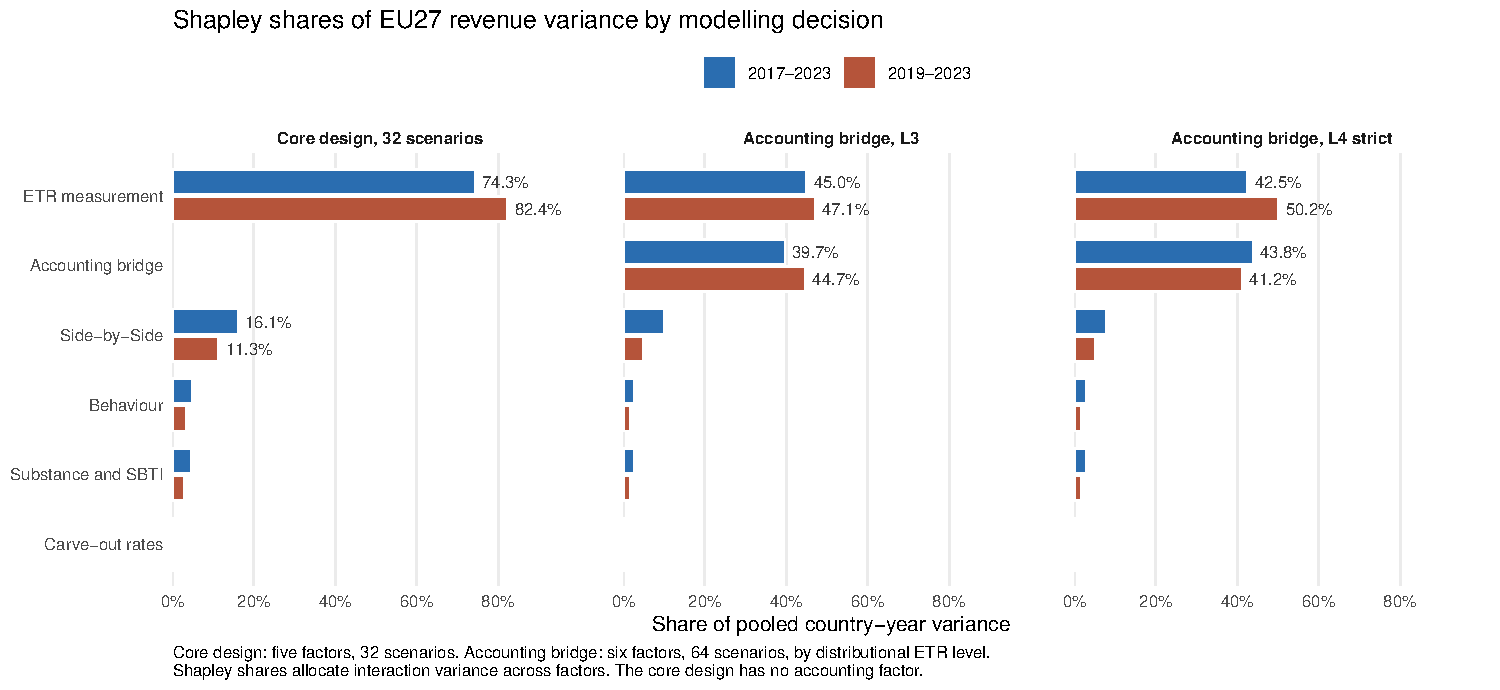
\includegraphics[width=\textwidth]{generated/paper_v2_figures/fig_v2_shapley_variance_core_and_accounting.pdf}
\caption{Shapley shares of the variance in EU27 revenue by modelling decision. Pooled country-year variance across scenarios. The left panel shows the core design (five decisions, 32 scenarios); the middle and right panels add the accounting bridge (six decisions, 64 scenarios) under the L3 and strict L4 measurement levels. Shares below 10\% are not labelled.}
\label{fig:v2_shapley_variance}
\end{figure}

% Generated by code/13_generate_exhibits.R
% Requires booktabs and array.
\begin{table}[htbp]
\centering
\footnotesize
\caption{Scenario and parameter uncertainty}\label{tab:tab_v2_main_table5_variance_and_uncertainty}
\begin{tabular}{@{}lllrr@{}}
\multicolumn{5}{@{}l}{\textbf{A1. Core 32-scenario factorial}} \\
\toprule
Window & Design & Factor & Main (\%) & Shapley (\%) \\
\midrule
2017–2023 & Core 32 & ETR & 72.17 & 74.67 \\
2017–2023 & Core 32 & Sectoral SBIE &  0.13 &  0.14 \\
2017–2023 & Core 32 & Rates &  0.14 &  0.19 \\
2017–2023 & Core 32 & SbS & 18.08 & 20.32 \\
2017–2023 & Core 32 & Behaviour &  4.32 &  4.68 \\
2019–2023 & Core 32 & ETR & 78.54 & 81.29 \\
2019–2023 & Core 32 & Sectoral SBIE &  0.07 &  0.08 \\
2019–2023 & Core 32 & Rates &  0.14 &  0.19 \\
2019–2023 & Core 32 & SbS & 12.97 & 15.43 \\
2019–2023 & Core 32 & Behaviour &  2.67 &  3.01 \\
2021–2023 & Core 32 & ETR & 82.76 & 85.36 \\
2021–2023 & Core 32 & Sectoral SBIE &  0.02 &  0.03 \\
2021–2023 & Core 32 & Rates &  0.14 &  0.19 \\
2021–2023 & Core 32 & SbS & 10.23 & 12.56 \\
2021–2023 & Core 32 & Behaviour &  1.57 &  1.85 \\
\bottomrule
\end{tabular}
\par\vspace{0.6em}
\begin{tabular}{@{}llllrrr@{}}
\multicolumn{7}{@{}l}{\textbf{A2. Accounting 64-scenario factorial}} \\
\toprule
Window & Design & ETR & Factor & Main (\%) & Shapley (\%) & Effect (US\$ bn) \\
\midrule
2017–2023 & Accounting 64 & L3 & ETR & 44.61 & 47.40 &  232.12 \\
2017–2023 & Accounting 64 & L3 & Sectoral SBIE &  0.05 &  0.09 &    3.04 \\
2017–2023 & Accounting 64 & L3 & Rates &  0.09 &  0.12 &    9.72 \\
2017–2023 & Accounting 64 & L3 & SbS & 10.36 & 11.85 &  -97.35 \\
2017–2023 & Accounting 64 & L3 & Behaviour &  2.24 &  2.60 &  -42.50 \\
2017–2023 & Accounting 64 & L3 & Accounting & 35.52 & 37.95 & -181.75 \\
2019–2023 & Accounting 64 & L3 & ETR & 46.16 & 49.42 &  168.78 \\
2019–2023 & Accounting 64 & L3 & Sectoral SBIE &  0.03 &  0.05 &    1.89 \\
2019–2023 & Accounting 64 & L3 & Rates &  0.08 &  0.11 &    7.10 \\
2019–2023 & Accounting 64 & L3 & SbS &  5.18 &  6.80 &  -58.74 \\
2019–2023 & Accounting 64 & L3 & Behaviour &  1.22 &  1.53 &  -25.53 \\
2019–2023 & Accounting 64 & L3 & Accounting & 38.83 & 42.08 & -141.93 \\
2017–2023 & Accounting 64 & L4 strict & ETR & 41.63 & 43.93 &  191.61 \\
2017–2023 & Accounting 64 & L4 strict & Sectoral SBIE &  0.06 &  0.11 &    2.66 \\
2017–2023 & Accounting 64 & L4 strict & Rates &  0.09 &  0.12 &    8.51 \\
2017–2023 & Accounting 64 & L4 strict & SbS &  8.73 & 10.16 &  -85.02 \\
2017–2023 & Accounting 64 & L4 strict & Behaviour &  2.35 &  2.72 &  -40.33 \\
2017–2023 & Accounting 64 & L4 strict & Accounting & 40.66 & 42.96 & -169.09 \\
2019–2023 & Accounting 64 & L4 strict & ETR & 48.14 & 50.79 &  163.85 \\
2019–2023 & Accounting 64 & L4 strict & Sectoral SBIE &  0.03 &  0.05 &    1.69 \\
2019–2023 & Accounting 64 & L4 strict & Rates &  0.07 &  0.10 &    6.68 \\
2019–2023 & Accounting 64 & L4 strict & SbS &  5.62 &  7.36 &  -58.84 \\
2019–2023 & Accounting 64 & L4 strict & Behaviour &  1.25 &  1.60 &  -26.51 \\
2019–2023 & Accounting 64 & L4 strict & Accounting & 37.50 & 40.10 & -131.34 \\
\bottomrule
\end{tabular}
\par\vspace{0.6em}
\begin{tabular}{@{}llrrrr@{}}
\multicolumn{6}{@{}l}{\textbf{B. Law of total variance, EU27}} \\
\toprule
Scope & Window & Scenario (\%) & Parameter (\%) & 90\% width (US\$ bn) & Proposal ratio \\
\midrule
EU27 & 2017–2023 & 98.77 &  1.23 & 55.13 &  8.65 \\
EU27 & 2019–2023 & 99.57 &  0.43 & 22.18 & 15.75 \\
\bottomrule
\end{tabular}
\par\vspace{0.6em}
\begin{minipage}{\textwidth}\footnotesize\raggedright\textit{Notes.} Panel A uses pooled EU27 country-year variation. The accounting design adds the CbCR-to-GloBE bridge as a sixth factor. Panel B uses 500 joint draws and 32 scenarios. The proposal ratio divides point scenario spread by the preferred scenario's 90\% parameter interval width. Split-SBTI, 32-scenario accounting, 2021–2023 accounting and member-state rows are in Online Appendix D. In this reference the SBTI axis is redundant: on and off cells agree exactly, so 64 diagnostic rows do not represent 64 varying policies. Historical six-factor capacity results remain separately reproducible.\end{minipage}
\end{table}


Panel A1 of Table \ref{tab:tab_v2_main_table5_variance_and_uncertainty} and the left panel of Figure \ref{fig:v2_shapley_variance} report the core design. Over 2017–2023, cumulative EU27 revenue ranges from \usd144.28 billion to \usd584.88 billion across the 32 scenarios; the preferred behavioural scenario gives \usd478.86 billion under universal allocation and \usd343.77 billion under SbS. ETR measurement ($x_1$) explains 71.46\% of the pooled variance as a main effect and 74.31\% by Shapley attribution. Its shares rise to 79.75\% and 82.39\% in 2019–2023 and to 84.54\% and 86.82\% in 2021–2023, as direct Table IV brackets replace imputation, so its dominance does not stem from the imputed early years. The SbS regime ($x_4$) comes second at 14.44\% and 16.07\% and lowers cumulative revenue by \usd98.61 billion on average. Behaviour ($x_5$, 4.52\% and 4.91\%), substance ($x_2$, 3.59\% and 4.53\%) and carve-out rates ($x_3$, 0.14\% and 0.18\%) are second-order. When $x_2$ is split in a separate design (Appendix \ref{app:decomposition}), the SBTI safe harbour carries a Shapley share of 6.20\% and the sectoral carve-out alone 0.24\%, so what little the substance decision moves comes from the incentive cap introduced in 2026.

The accounting bridge reorders the ranking below the top (Panel A2). Under L3 over 2017–2023, ETR measurement accounts for 41.80\% of the variance as a main effect and 45.02\% by Shapley attribution, and it raises cumulative revenue by \usd194.09 billion on average. The bridge accounts for 36.89\% and 39.66\% and lowers revenue by \usd153.66 billion on average, taking the preferred SbS scenario from \usd343.77 billion to \usd214.06 billion. In 2019–2023 the Shapley shares are 47.08\% for measurement and 44.67\% for accounting. Under strict L4, accounting carries 43.82\% and 41.23\% in the two windows, against 42.49\% and 50.18\% for measurement. Jointly, the two decisions about the tax base explain 84.68–91.75\% of the variance across windows and levels, and more than 93\% in 2021–2023.

The two base decisions dominate in different places (Appendix \ref{app:decomposition}). Under L3 over 2017–2023, measurement carries a Shapley share of 77.24\% in Germany and 65.69\% in France, the large high-tax real economies, against 10.55\% and 13.47\% for the bridge. The bridge dominates in conduit and investment hubs: 73.74\% in Luxembourg, 56.13\% in Ireland and, under strict L4, 46.96\% in the Netherlands. In these hubs most profit is taxed below 15\% however the rate is measured, so the size of the base after dividends and losses decides the outcome. A large spread across scenarios matters only if it exceeds the noise in the estimated parameters, which the next subsection checks.

\subsection{Scenario disagreement versus statistical noise}\label{sec:uncertainty}

Some of the spread across estimates could come from the statistical uncertainty in estimated inputs, and the analysis measures that share directly. Two kinds of uncertainty are at stake. Disagreement across scenarios is epistemic: it reflects discrete modelling and legal choices $x$ on which analysts differ, and agreement can remove it. Noise in estimated inputs is aleatoric: it reflects estimation error in the continuous parameters $\theta=(\hat\beta_1,\hat\rho_{pt},\varepsilon^{\mathrm{Stage1}}_{jt})$, the behavioural slope, the profit-correction rates and the residuals of the fitted ETR distributions, and it would remain if every analyst chose the same $x$ \citep{hullermeier2021}. If the second kind were large, the ranking in Section \ref{sec:factorial} could reflect noise.

The decomposition below takes simulated EU27 revenue under 500 joint draws of $\theta$, each evaluated in all 32 core scenarios, and produces the scenario and parameter shares of total variance and a ratio $\Lambda$ that compares the two on the scale of the forecast; Panel B of Table \ref{tab:tab_v2_main_table5_variance_and_uncertainty} reports both, and Section \ref{sec:conclusion} returns to them:
\begin{equation}\label{eq:totalvariance}
\operatorname{Var}(R)=\underbrace{\operatorname{Var}_x\!\bigl(\mathbb{E}_\theta[R\mid x]\bigr)}_{\text{scenario variance}}+\underbrace{\mathbb{E}_x\!\bigl[\operatorname{Var}_\theta(R\mid x)\bigr]}_{\text{parameter variance}},\qquad
\Lambda=\frac{\max_x\hat R(x)-\min_x\hat R(x)}{W_{90}(x^{\star})}.
\end{equation}
$R$ is cumulative EU27 revenue over the window and $\hat R(x)$ its value at the point estimates. $x^{\star}$ is the preferred scenario (distributional measurement, aggregate carve-out at initial rates, SbS and behaviour), and $W_{90}(x^{\star})$ is the width of its simulated 90\% parameter interval. A ratio above one means that moving between defensible scenarios shifts the estimate by more than parameter noise does within the preferred one. The joint Monte Carlo decomposition and $\Lambda$, labelled the proposal ratio in Table \ref{tab:tab_v2_main_table5_variance_and_uncertainty}, are introduced in this paper.\footnote{The draws cover the three estimated inputs in $\theta$ and the 32 core scenarios. The inputs of the accounting bridge and the legal status of each jurisdiction stay at their frozen values, so the parameter share measures the noise in estimated inputs only.}

Parameter uncertainty is small. It accounts for 1.71\% of the variance in cumulative EU27 revenue over 2017–2023, against 98.29\% for scenario choices, and for 0.36\% over 2019–2023, against 99.64\%. The spread across scenarios, \usd440.60 billion and \usd310.44 billion, exceeds the 90\% parameter interval, \usd63.61 billion and \usd20.71 billion wide, by factors of $\Lambda=6.93$ and $\Lambda=14.99$.

A Shapley attribution of the parameter variance shows where the remaining noise comes from. Over 2017–2023 the residuals of the fitted ETR distributions (Section \ref{sec:etr_validation}) explain 78.58\% of it, the slope $\hat\beta_1$ 11.90\% and the profit correction $\hat\rho_{pt}$ 9.53\%. The residuals weigh heavily because the 2017–2018 distributions are transported back from later years (Section \ref{sec:etr_ladder}). Over 2019–2023, with direct Table IV brackets in place of that backcasting, their share falls to 0.01\%, leaving the profit correction (59.71\%) and the slope (40.28\%). The result holds state by state (Appendix \ref{app:decomposition}): the ratio $\Lambda_c$ exceeds one in all 22 collecting states in both windows, and parameter variance exceeds scenario variance only in Austria over 2017–2023, at 52.89\% of the total. Scenario disagreement dominates, so the remaining test is whether any scenario reproduces what governments expect to collect.

\subsection{Back-testing against national budgets}\label{sec:backtest}

National budgets give an outside check on the model, because finance ministries forecast what they expect to collect from the same rules. A model and a forecast can agree for the wrong reasons, so the comparison is made at each stage of the accounting bridge. It uses the forecasts of the eight Member States in Section \ref{sec:otherdata}, matched to the channel each covers where the source allows, and two windows: fiscal year 2023 and the annual average over 2019–2023.\footnote{National forecasts are cash or accrual estimates for specific budget years, some net of implementation costs, and they reflect elections and safe harbours that groups make firm by firm, which aggregated country-by-country cells cannot observe. The Dutch post-package figure is inferred from published components, and the safe harbour screen is a proxy. The comparison is therefore a structural diagnostic of where the gap arises and makes no claim to be a point forecast.}

% Generated by code/13_generate_exhibits.R
% Requires booktabs and array.
\begin{table}[htbp]
\centering
\footnotesize
\caption{National budget benchmarks and accounting waterfall}\label{tab:tab_v2_budget_backtest_and_hanlon_waterfall}
\begin{tabular}{@{}lllrrr@{}}
\multicolumn{6}{@{}l}{\textbf{A. Official benchmarks and modelled revenue ranges}} \\
\toprule
ISO & Window & Budget basis & Benchmark & L3 (16) & Core (32) \\
\midrule
NLD & FY2023 & structural, 2020–2023 CbCR base & 0.1760 & 7.0875–12.8004 & 0.2536–12.8004 \\
DEU & FY2023 & 2026 cash & 1.0000 & 6.6360–14.3544 & 0.7600–14.3544 \\
FRA & FY2023 & 2026 cash & 0.5000 & 2.0530–6.5324 & 0.2072–6.5324 \\
IRL & FY2023 & 2026 cash & 3.2000 & 5.7114–10.7257 & 5.2687–10.7257 \\
LUX & FY2023 & 2026 cash & 0.0800 & 4.3902–6.4497 & 3.7496–6.4497 \\
BEL & FY2023 & 2024 cash & 0.6340 & 0.9456–1.1254 & 0.0046–1.1254 \\
AUT & FY2023 & 2026 onward & 0.1000 & 0.4969–1.1340 & 0.4275–1.1340 \\
SVK & FY2023 & 2026 state budget & 0.0485 & 0.0365–0.0407 & 0.0000–0.0407 \\
NLD & 2019–2023 & structural, 2020–2023 CbCR base & 0.1760 & 10.9697–17.5367 & 5.9851–17.5367 \\
DEU & 2019–2023 & 2026 cash & 1.0000 & 7.3289–15.2432 & 0.8989–15.2432 \\
FRA & 2019–2023 & 2026 cash & 0.5000 & 3.2387–8.9105 & 0.3059–8.9105 \\
IRL & 2019–2023 & 2026 cash & 3.2000 & 5.8033–10.0016 & 5.4165–10.0016 \\
LUX & 2019–2023 & 2026 cash & 0.0800 & 6.4505–10.1894 & 5.5640–10.1894 \\
BEL & 2019–2023 & 2024 cash & 0.6340 & 1.4135–1.7985 & 0.1534–1.7985 \\
AUT & 2019–2023 & 2026 onward & 0.1000 & 0.7195–1.2058 & 0.6451–1.2058 \\
SVK & 2019–2023 & 2026 state budget & 0.0485 & 0.0527–0.0627 & 0.0527–0.1722 \\
\bottomrule
\end{tabular}
\par\vspace{0.6em}
\begin{tabular}{@{}llrrrrrr@{}}
\multicolumn{8}{@{}l}{\textbf{B. Preferred SbS collector revenue after each adjustment}} \\
\toprule
ISO & Window & Baseline & Dividends & Current losses & Prior losses & Tax envelope & 2026 screen \\
\midrule
NLD & FY2023 &  7.088 & 5.512 & 3.079 & 2.810 & 2.544 & 0.447 \\
NLD & 2019–2023 & 10.970 & 9.356 & 6.261 & 5.963 & 5.427 & 3.428 \\
DEU & FY2023 &  6.636 & 5.455 & 4.010 & 3.779 & 3.426 & 0.526 \\
DEU & 2019–2023 &  7.329 & 6.310 & 4.914 & 4.766 & 4.025 & 1.039 \\
FRA & FY2023 &  2.053 & 1.992 & 1.484 & 1.416 & 1.053 & 0.173 \\
FRA & 2019–2023 &  3.239 & 2.716 & 2.025 & 1.960 & 1.185 & 0.216 \\
IRL & FY2023 &  5.712 & 5.632 & 4.716 & 4.540 & 3.775 & 3.586 \\
IRL & 2019–2023 &  5.868 & 5.766 & 4.584 & 4.460 & 4.061 & 2.934 \\
LUX & FY2023 &  4.390 & 3.544 & 1.487 & 1.135 & 1.090 & 0.747 \\
LUX & 2019–2023 &  6.450 & 5.621 & 2.031 & 1.293 & 1.149 & 0.874 \\
BEL & FY2023 &  1.052 & 1.027 & 0.639 & 0.615 & 0.563 & 0.143 \\
BEL & 2019–2023 &  1.636 & 1.505 & 1.097 & 1.068 & 0.850 & 0.373 \\
AUT & FY2023 &  0.497 & 0.495 & 0.397 & 0.375 & 0.058 & 0.041 \\
AUT & 2019–2023 &  0.719 & 0.672 & 0.563 & 0.539 & 0.433 & 0.290 \\
SVK & FY2023 &  0.037 & 0.037 & 0.034 & 0.034 & 0.000 & 0.000 \\
SVK & 2019–2023 &  0.053 & 0.053 & 0.046 & 0.046 & 0.021 & 0.007 \\
\bottomrule
\end{tabular}
\par\vspace{0.6em}
\begin{minipage}{\textwidth}\footnotesize\raggedright\textit{Notes.} EUR bn per year, converted at 1.0813 USD per EUR. Panel A spans both policy regimes. L3 fixes distributional ETR measurement, and the core adds the average ETR scenarios. Slovakia is QDMTT only. Belgium is QDMTT plus IIR, with the official amount net of costs. The Dutch after-package amount is inferred from published components. The two model windows apply later rules to historical activity. Panel B holds the scenario fixed. Its cumulative 2026 safe harbour screen uses the net CbCR profit and tax envelope.\end{minipage}
\end{table}


Panel A of Table \ref{tab:tab_v2_budget_backtest_and_hanlon_waterfall} sets each benchmark against the range of the 32 core scenarios; in FY2023 even the lowest scenario exceeds the benchmark everywhere except Slovakia. The first column of Panel B gives the preferred SbS scenario under L3 before any accounting adjustment, and it overshoots by multiples: \EUR6.68 billion against a direct post-package benchmark of \EUR0.18 billion for the Netherlands, \EUR4.25 billion against \EUR0.08 billion for Luxembourg, \EUR6.28 billion against \EUR1.00 billion in cash and \EUR0.20 billion in full-year effect for Germany, \EUR1.86 billion against \EUR0.50 billion for France and \EUR5.32 billion against \EUR3.20 billion for Ireland. Bilateral cell averages (L2), close to the coarse aggregation behind many ministry forecasts, land near the cash forecasts for Germany (\EUR0.995 billion against \EUR1.000 billion in FY2023) and Belgium (\EUR0.634 billion a year over 2019–2023 against \EUR0.634 billion). The agreement comes from offsetting errors: averaging hides low-taxed profit (Section \ref{sec:etr_ladder}), while the unadjusted base inflates it.

Panel B applies the adjustments one at a time. The first three are the steps of the accounting bridge in Section \ref{sec:accounting_bridge}: the dividend purge, current loss netting and prior loss carryforward. The fourth replaces tax accrued with the covered-tax envelope $\max\{\theta^{\mathrm{accrued}}_{pjt},\theta^{\mathrm{paid}}_{pjt}\}$, a public-data proxy for covered taxes, which include deferred tax that the accrued figure omits. The fifth removes cells that would pass the Transitional CbCR Safe Harbour for 2024–2026 (a de minimis, simplified ETR or routine profits test), at the 2026 simplified ETR threshold of 17\%. Summed over all EU27 collectors, FY2023 revenue falls from \EUR36.39 billion to \EUR30.29 billion after the dividend purge, \EUR21.35 billion after current losses, \EUR20.15 billion after prior losses, \EUR16.22 billion after the tax envelope and \EUR7.99 billion after the safe harbour screen, or \EUR14.35 billion without its simplified ETR test.

\begin{figure}[htbp]
\centering
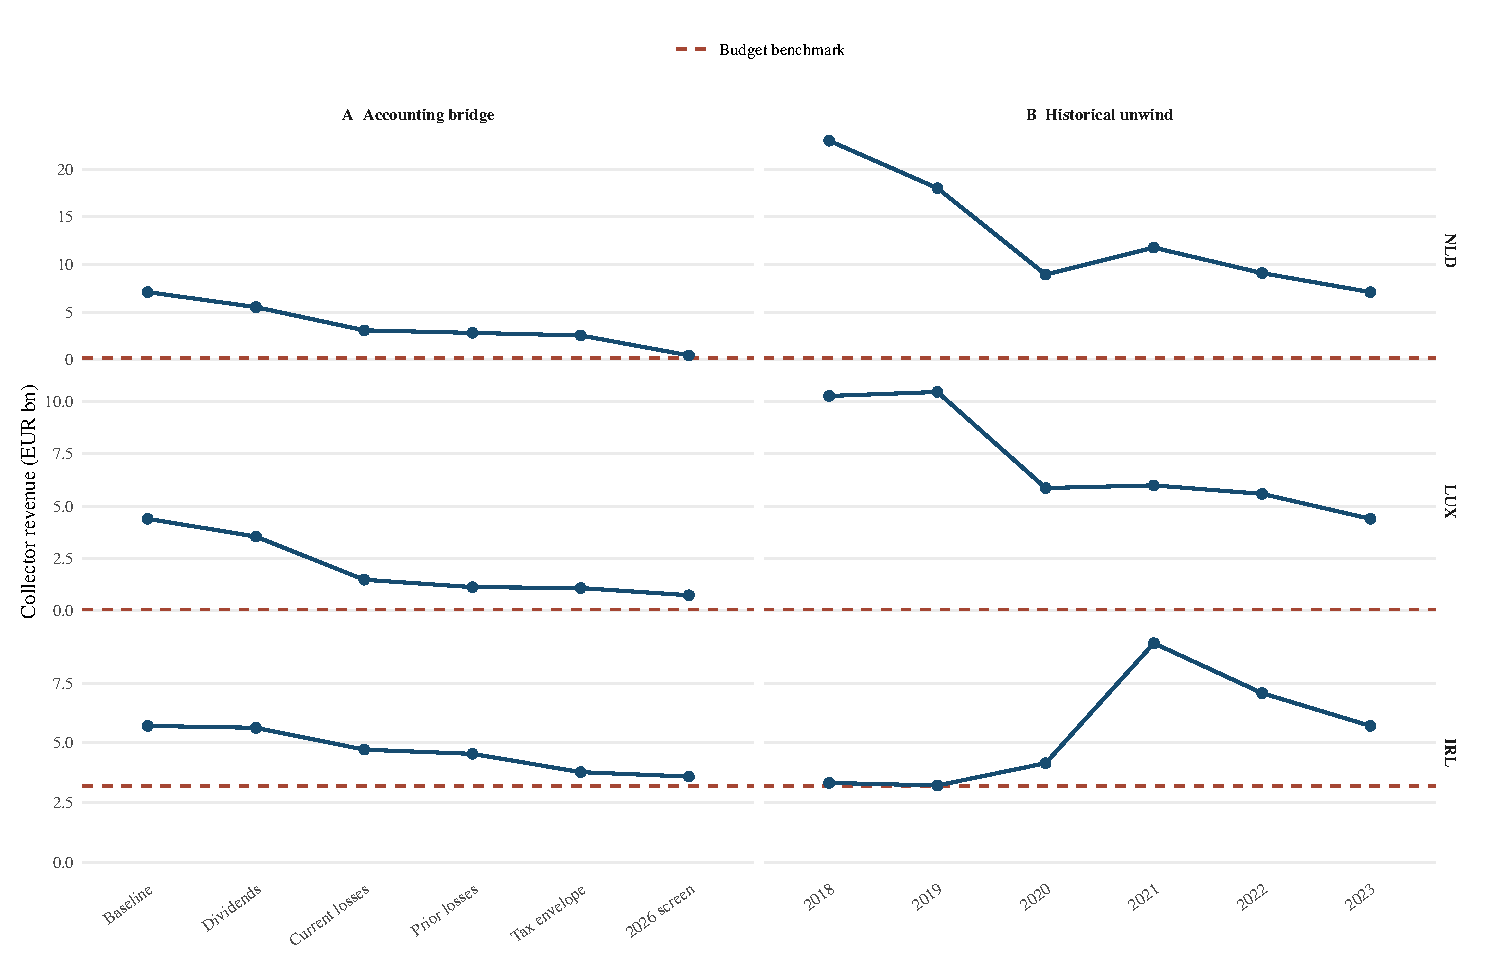
\includegraphics[width=\textwidth]{generated/paper_v2_figures/fig_v2_cbcr_to_budget_waterfall.pdf}
\caption{From country-by-country liability to national budget benchmarks. Panel A applies the adjustments of Table \ref{tab:tab_v2_budget_backtest_and_hanlon_waterfall}, Panel B, to FY2023 collector revenue in the preferred SbS scenario. Panel B shows annual modelled collector revenue in the same scenario, 2018–2023. Dashed lines mark each state's budget benchmark, which refers to a separate fiscal period and definition.}
\label{fig:v2_budget_waterfall}
\end{figure}

Two results stand out. First, for the six collectors outside the conduit hubs, the FY2023 gap after the full sequence is below \EUR0.5 billion. Ireland lands at \EUR3.538 billion against its forecast of \EUR3.200 billion, and Germany, at \EUR0.514 billion, lies between its full-year effect of \EUR0.200 billion and its 2026 cash estimate of \EUR1.000 billion. France reaches \EUR0.185 billion against \EUR0.500 billion, Belgium \EUR0.144–0.553 billion (with and without the screen) against \EUR0.634 billion, Austria \EUR0.008 billion against \EUR0.100 billion and Slovakia zero against \EUR0.048 billion. For these states the gap between the raw model and the budget is a matter of the tax base, as Section \ref{sec:factorial} predicts.

Second, the sequence lowers Dutch FY2023 collector revenue by 93.7\%, from \EUR6.684 billion to \EUR0.419 billion (\EUR0.362 billion of it domestic top-up tax), against a direct post-package benchmark of \EUR0.176 billion; Luxembourg falls from \EUR4.250 billion to \EUR0.705 billion against \EUR0.080 billion. The 2019–2023 average still leaves \EUR3.355 billion for the Netherlands, because the conduit base shrank before the tax took effect. Low-taxed profit booked in the two countries fell by 64.7\% between 2018 and 2023, from \usd222.59 billion to \usd78.20 billion in the Netherlands and from \usd105.21 billion to \usd37.55 billion in Luxembourg. The fall followed the anti-hybrid rules of the second EU Anti-Tax Avoidance Directive from 2020, the Dutch conditional withholding tax on interest and royalties from 2021, and the unwinding of CV/BV structures before 2024. Panel B of Figure \ref{fig:v2_budget_waterfall} shows the matching fall in modelled collector revenue, from \EUR22.76 billion to \EUR6.68 billion in the Netherlands and from \EUR10.25 billion to \EUR4.25 billion in Luxembourg. Pooling earlier vintages therefore projects dismantled conduit structures into post-2024 budgets. Section \ref{sec:allocation} turns from the size of revenue to the question of which treasuries collect it and what incentives that creates.

\section{Who collects and who gives up revenue}\label{sec:allocation}

Once the size of the top-up liability is settled, the legal order of claims and the relocation of profit by firms decide which treasuries receive it, and whether a host state has any reason to keep its own domestic top-up tax. Section \ref{sec:ledger} sets the liability generated in each Member State against the revenue its treasury collects, Section \ref{sec:cit_recovery} adds the ordinary corporate tax that relocated profit pays, and Section \ref{sec:repeal_game} tests whether any state gains by repealing its domestic top-up tax.

\subsection{Liability generated and revenue collected}\label{sec:ledger}

The state where low-taxed profit is booked does not always collect the tax that profit generates. The host has the first claim only if it levies a QDMTT; otherwise the claim passes to the parent's state, then to the other states in which the group operates, and since January 2026 it lapses for groups parented in the United States. Revenue in one Member State therefore depends on the legislation of others.

The waterfall below takes the post-behaviour liability $L_{pjt}$ of equation \eqref{eq:liability}, splits it into four pools and returns the revenue of each collector, which defines the shares $a_{c\mid pjt}$ of equation \eqref{eq:revenue} and the entries of Table \ref{tab:tab_v2_main_table7_source_collector_ledger}:
\begin{align}
L_{pjt} &= L^{Q}_{pjt} + L^{I}_{pjt} + L^{U}_{pjt} + L^{S}_{pjt}, \label{eq:waterfall}\\
R_c &= \sum_{p,j,t}\Bigl(\mathbb{1}\{j=c\}\,L^{Q}_{pjt} + \mathbb{1}\{p=c\}\,L^{I}_{pjt} + \omega^{U}_{cpt}\,L^{U}_{pjt}\Bigr). \label{eq:collectors}
\end{align}
The host pool $L^{Q}_{pjt}$ takes the whole liability when host $j$ levies a qualified QDMTT; failing that, the parent pool $L^{I}_{pjt}$ takes it when parent state $p$ applies a qualified IIR. $L^{S}_{pjt}$ holds the liability of US-parented groups in hosts without a QDMTT, which SbS extinguishes. The remainder $L^{U}_{pjt}$ goes to the states that apply a UTPR and host the group, weighted equally by its employees and tangible assets there ($\omega^{U}_{cpt}$). Legal status follows the sources in Section \ref{sec:otherdata}.

Applied to every Member State, the waterfall yields a source–collector fiscal flow ledger, introduced in this paper, which sets the liability that profit booked in each state generates against the revenue its treasury collects. Four institutional regime groups, also our own, sort the states by the legal position behind the gap. High-salience sources (group 1) generate liability above a quarter of their cumulative corporate income tax (CIT) revenue. QDMTT-protected collectors (group 2) raise at least three quarters of their receipts through the QDMTT, and residual IIR and UTPR collectors (group 3) rely more on the other rules. Article 50 fiscal exporters (group 4) deferred the IIR and UTPR without enacting a QDMTT.\footnote{The thesis grouped the states by four-cluster $k$-means on the principal components of their revenue channel shares. With 27 observations the clusters were unstable, and the shares of the five states that collect nothing are undefined and had to be filled with medians. Appendix \ref{app:allocation} reports the legacy components and cluster stability tables.}

% Generated by code/13_generate_exhibits.R
% Requires booktabs and array.
\begin{table}[htbp]
\centering
\scriptsize
\caption{Source liability and collector receipts}\label{tab:tab_v2_main_table7_source_collector_ledger}
\begin{tabular}{@{}llrrrrrr@{}}
\multicolumn{8}{@{}l}{\textbf{A. Liability generated and routed from source}} \\
\toprule
ISO & Group & Generated & Retained & IIR abroad & UTPR abroad & SbS relief & Unassigned \\
\midrule
CYP & 1 &  6.51 &  0.00 & 1.94 & 0.37 & 4.20 & 0.00 \\
HUN & 1 &  5.47 &  5.47 & 0.00 & 0.00 & 0.00 & 0.00 \\
LUX & 1 & 51.82 & 51.82 & 0.00 & 0.00 & 0.00 & 0.00 \\
MLT & 1 &  4.94 &  0.00 & 2.17 & 0.08 & 2.68 & 0.00 \\
NLD & 1 & 86.50 & 86.50 & 0.00 & 0.00 & 0.00 & 0.00 \\
BEL & 2 & 10.64 & 10.64 & 0.00 & 0.00 & 0.00 & 0.00 \\
DNK & 2 &  6.48 &  6.48 & 0.00 & 0.00 & 0.00 & 0.00 \\
FIN & 2 &  2.34 &  2.34 & 0.00 & 0.00 & 0.00 & 0.00 \\
IRL & 2 & 28.75 & 28.75 & 0.00 & 0.00 & 0.00 & 0.00 \\
SVK & 2 &  0.45 &  0.45 & 0.00 & 0.00 & 0.00 & 0.00 \\
AUT & 3 &  3.41 &  3.41 & 0.00 & 0.00 & 0.00 & 0.00 \\
BGR & 3 &  0.86 &  0.86 & 0.00 & 0.00 & 0.00 & 0.00 \\
CZE & 3 &  1.26 &  1.26 & 0.00 & 0.00 & 0.00 & 0.00 \\
DEU & 3 & 28.20 & 28.20 & 0.00 & 0.00 & 0.00 & 0.00 \\
ESP & 3 & 12.29 & 12.29 & 0.00 & 0.00 & 0.00 & 0.00 \\
FRA & 3 & 13.05 & 13.05 & 0.00 & 0.00 & 0.00 & 0.00 \\
GRC & 3 &  1.40 &  1.40 & 0.00 & 0.00 & 0.00 & 0.00 \\
HRV & 3 &  0.31 &  0.31 & 0.00 & 0.00 & 0.00 & 0.00 \\
ITA & 3 &  6.40 &  6.40 & 0.00 & 0.00 & 0.00 & 0.00 \\
POL & 3 &  2.00 &  2.00 & 0.00 & 0.00 & 0.00 & 0.00 \\
PRT & 3 &  0.83 &  0.83 & 0.00 & 0.00 & 0.00 & 0.00 \\
ROU & 3 &  0.94 &  0.94 & 0.00 & 0.00 & 0.00 & 0.00 \\
SVN & 3 &  0.38 &  0.38 & 0.00 & 0.00 & 0.00 & 0.00 \\
SWE & 3 &  4.35 &  4.35 & 0.00 & 0.00 & 0.00 & 0.00 \\
EST & 4 &  0.25 &  0.00 & 0.23 & 0.00 & 0.02 & 0.00 \\
LTU & 4 &  0.14 &  0.00 & 0.02 & 0.04 & 0.08 & 0.00 \\
LVA & 4 &  0.11 &  0.00 & 0.08 & 0.01 & 0.02 & 0.00 \\
\bottomrule
\end{tabular}
\par\vspace{0.6em}
\begin{tabular}{@{}lrrrrrrrr@{}}
\multicolumn{9}{@{}l}{\textbf{B. Collector receipts, ordinary CIT and scenario spread}} \\
\toprule
ISO & QDMTT & IIR & UTPR & Collected & Net & Rule B CIT & CIT (\%) & Spread \\
\midrule
CYP &  0.00 &  0.00 &  0.34 &  0.34 & -6.16 &  0.00 &   2.95 &   0.53 \\
HUN &  5.47 &  0.00 &  1.20 &  6.67 &  1.20 &  0.00 &  34.78 &   8.50 \\
LUX & 51.82 &  3.91 &  2.09 & 57.81 &  5.99 &  0.39 & 212.21 &  49.97 \\
MLT &  0.00 &  0.00 &  0.00 &  0.00 & -4.94 &  0.43 &   0.00 &   0.00 \\
NLD & 86.50 &  2.51 &  9.28 & 98.30 & 11.80 &  3.49 &  36.84 & 100.52 \\
BEL & 10.64 &  1.07 &  1.75 & 13.46 &  2.82 &  6.86 &   8.90 &  23.56 \\
DNK &  6.48 &  0.91 &  0.77 &  8.17 &  1.69 &  1.41 &   9.41 &  10.78 \\
FIN &  2.34 &  0.00 &  0.30 &  2.64 &  0.30 &  0.49 &   5.12 &   3.85 \\
IRL & 28.75 &  0.00 &  9.17 & 37.92 &  9.17 &  0.00 &  32.89 &  39.10 \\
SVK &  0.45 &  0.00 &  0.00 &  0.45 &  0.00 &  0.40 &   1.66 &   0.94 \\
AUT &  3.41 &  0.00 &  1.35 &  4.77 &  1.35 &  2.05 &   5.28 &   3.99 \\
BGR &  0.86 &  0.00 &  0.44 &  1.30 &  0.44 &  0.00 &   9.35 &   1.97 \\
CZE &  1.26 &  0.00 &  1.18 &  2.45 &  1.18 &  1.41 &   3.34 &   5.60 \\
DEU & 28.20 & 14.13 & 13.97 & 56.30 & 28.10 & 16.56 &   9.44 & 106.67 \\
ESP & 12.29 &  4.27 &  4.21 & 20.77 &  8.48 &  7.53 &   8.58 &  34.39 \\
FRA & 13.05 &  6.04 &  5.15 & 24.23 & 11.18 &  9.51 &   5.40 &  62.48 \\
GRC &  1.40 &  0.17 &  0.31 &  1.88 &  0.47 &  0.76 &   5.87 &   2.86 \\
HRV &  0.31 &  0.00 &  0.38 &  0.69 &  0.38 &  0.28 &   5.95 &   0.76 \\
ITA &  6.40 &  2.88 &  4.41 & 13.69 &  7.29 &  8.02 &   4.30 &  26.19 \\
POL &  2.00 &  0.00 &  2.39 &  4.39 &  2.39 &  0.57 &   4.09 &  12.47 \\
PRT &  0.83 &  0.10 &  0.58 &  1.51 &  0.68 &  1.93 &   2.81 &   2.89 \\
ROU &  0.94 &  0.81 &  1.68 &  3.43 &  2.49 &  1.12 &   8.05 &   5.91 \\
SVN &  0.38 &  0.02 &  0.85 &  1.25 &  0.87 &  0.24 &  14.50 &   1.64 \\
SWE &  4.35 &  0.00 &  3.28 &  7.63 &  3.28 &  1.70 &   6.12 &  10.89 \\
EST &  0.00 &  0.00 &  0.00 &  0.00 & -0.25 &  0.05 &   0.00 &   0.00 \\
LTU &  0.00 &  0.00 &  0.00 &  0.00 & -0.14 &  0.00 &   0.00 &   0.00 \\
LVA &  0.00 &  0.00 &  0.00 &  0.00 & -0.11 &  0.07 &   0.00 &   0.00 \\
\bottomrule
\end{tabular}
\par\vspace{0.6em}
\begin{minipage}{\textwidth}\footnotesize\raggedright\textit{Notes.} Cumulative 2017–2023, US\$ bn, preferred behavioural SbS scenario. Net is collected minus source liability. Rule B CIT is gross induced ordinary CIT. Groups are high-salience sources (1), QDMTT-protected collectors (2), residual IIR/UTPR collectors (3), and Article 50 fiscal exporters (4). Unassigned is residual UTPR liability outside observed parent-year routing support. The UTPR collector map uses verified national applicability. R1, R2 and R3 vary source QDMTT and parent IIR. Qualification sensitivities are in Online Appendix E.\end{minipage}
\end{table}


Over 2017–2023, in the preferred behavioural SbS scenario, profit booked in EU27 affiliates generates \usd280.10 billion of top-up liability, while EU27 treasuries collect \usd343.77 billion: \usd268.15 billion through QDMTTs, \usd36.82 billion through IIRs and \usd38.80 billion through UTPRs. The Union is thus a net importer of \usd63.67 billion. Under universal allocation, collector revenue rises to \usd478.86 billion, with \usd173.89 billion from UTPRs.

Five Member States collect nothing (Cyprus, Malta, Estonia, Lithuania and Latvia), although they host \usd117.73 billion of corrected positive profit over 2017–2023. That profit generates \usd11.94 billion of liability: \usd6.51 billion in Cyprus, \usd4.94 billion in Malta, \usd0.25 billion in Estonia, \usd0.14 billion in Lithuania and \usd0.11 billion in Latvia. Foreign IIRs collect \usd4.44 billion of it, foreign UTPRs \usd0.51 billion, and SbS extinguishes \usd6.99 billion. The cause is legal. Estonia, Latvia, Lithuania and Malta elected the six-year deferral of the IIR and UTPR under Article 50 of the EU minimum tax directive and enacted no QDMTT. Cyprus enacted an IIR and a domestic top-up tax in Law 151(I)/2024, which had not completed transitional qualification in the Central Record of 1 May 2026. Its 2023 liability equals 177.86\% of its CIT revenue, and treating the law as qualified would keep \usd5.74 billion in Cyprus (Appendix \ref{app:allocation}).

\begin{figure}[htbp]
\centering
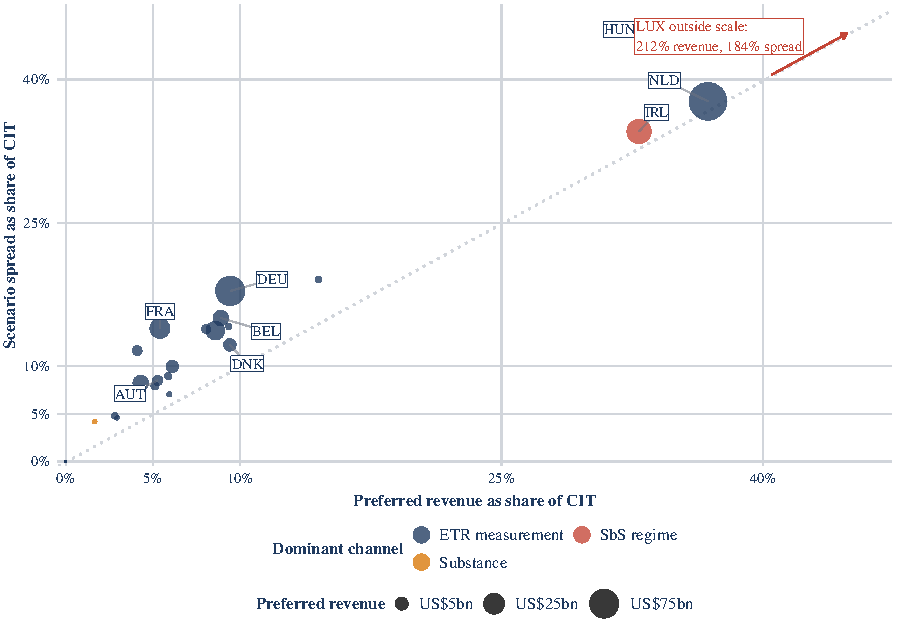
\includegraphics[width=\textwidth]{generated/figures/fig_country_salience_uncertainty.pdf}
\caption{Fiscal salience and scenario uncertainty by Member State. The horizontal axis gives collector revenue in the preferred behavioural SbS scenario as a share of CIT revenue, cumulative over 2017–2023; the vertical axis gives the range of collector revenue across the 32 core scenarios on the same scale. Marker size is collector revenue, and colour marks the decision with the largest main effect in each state. The dotted line marks equal values. Luxembourg lies outside the plotted range.}
\label{fig:v2_country_salience}
\end{figure}

Panel A and Figure \ref{fig:v2_country_salience} show how far receipts and liability diverge. Where the QDMTT is in force, group 1 keeps its liability, and the sums are large relative to its budget: receipts equal 207.45\% of CIT revenue in Luxembourg, 35.48\% in the Netherlands and 31.99\% in Hungary, with scenario spreads of the same order. Malta and Cyprus collect nothing, although the liability booked there equals 82.68\% and 55.99\% of their CIT revenue. In group 2 (Austria, Belgium, Denmark, Finland, Greece, Ireland and Slovakia) the QDMTT keeps at least three quarters of receipts at home; Ireland's liability, at 24.93\% of CIT revenue, lies just below the salience threshold. Group 3 hosts the parents and the real activity on which the IIR and UTPR draw, and so collects more than its own profit generates: Germany \usd51.26 billion against \usd28.20 billion, a net import of \usd23.06 billion, and France \usd22.28 billion against \usd13.05 billion. The Baltic states of group 4 export all of their liability. Firms' responses move profit between these states, and the next subsection counts the ordinary tax that the move brings.

\subsection{What behaviour costs and what it brings home}\label{sec:cit_recovery}

When firms move profit out of low-tax countries, the lost top-up tax is partly replaced by ordinary corporate tax wherever the profit lands. Profit that leaves an affiliate taxed below 15\% stops generating top-up tax but pays CIT where it is booked, and the source loses the low ordinary tax it levied, so counting only the forgone top-up tax misstates what behaviour costs.

The destination of relocated profit is unobserved, so a rule must assign it. Rule B sends it to where the same group has real activity and adapts the formulary weights of \citet{garcia-bernardo2024} in two ways: destinations are restricted to affiliates of the same parent, and eligibility follows from tax rates alone, without a list of conduit countries. The equations below take the profit $\Delta\pi_{pjt}$ that leaves low-taxed cell $(p,j,t)$, assign it to destinations $d$ and give each state's gross and net ordinary tax recovery (Panel B of Table \ref{tab:tab_v2_main_table7_source_collector_ledger}):
\begin{gather}
\omega^{B}_{d\mid pjt} = \frac{1}{4}\,\frac{E_{pdt}}{\sum_{k\in D_{pjt}}E_{pkt}} + \frac{1}{4}\,\frac{W_{pdt}}{\sum_{k\in D_{pjt}}W_{pkt}} + \frac{1}{2}\,\frac{Y_{pdt}}{\sum_{k\in D_{pjt}}Y_{pkt}},\qquad d\in D_{pjt}, \label{eq:ruleb}\\
\mathrm{CIT}^{\mathrm{gross}}_{d} = \sum_{p,j,t}\tau^{\mathrm{stat}}_{dt}\,\omega^{B}_{d\mid pjt}\,\Delta\pi_{pjt}, \qquad
\mathrm{CIT}^{\mathrm{net}}_{c} = \mathrm{CIT}^{\mathrm{gross}}_{c} - \sum_{p,t}\tau_{pct}\,\Delta\pi_{pct}. \label{eq:citrecovery}
\end{gather}
$E$, $W$ and $Y$ are the employees, payroll and unrelated-party revenue of parent $p$'s affiliate in $d$. The eligible set $D_{pjt}$ contains the parent's other affiliates whose host has a statutory rate $\tau^{\mathrm{stat}}_{dt}$ of at least 15\% and an ETR above that of the source. The second term of the net recovery is the ordinary tax that source $c$ loses at the low ETR $\tau_{pct}$ of the departing profit.\footnote{Where a parent has no eligible affiliate, the profit is allocated by the global activity of eligible destinations in the same year. Appendix \ref{app:allocation} compares Rule B with Rule A, which pools each parent's relocated profit and excludes a list of conduit countries, and with Rule C, which sends half of it to the parent's headquarters.}

Across the EU27 over 2017–2023, in the preferred SbS scenario, switching on the behavioural response lowers direct top-up tax by \usd58.09 billion, from \usd401.86 billion to \usd343.77 billion. Relocated profit raises gross ordinary CIT in EU27 destinations by \usd65.27 billion, a gross fiscal change of $+$\usd7.18 billion. Low-tax EU27 affiliates lose \usd17.11 billion of ordinary CIT on the profit that leaves, so net recovery is \usd48.15 billion and the net fiscal change is $-$\usd9.94 billion.

The incidence is sharply asymmetric. Large destination economies gain on balance: Germany loses \usd7.53 billion of top-up tax and \usd2.50 billion of source CIT but gains \usd16.56 billion of ordinary CIT, a net \usd6.53 billion, and the net gains are \usd5.66 billion in Italy, \usd5.14 billion in France, \usd4.00 billion in Belgium and \usd3.51 billion in Spain. Low-tax hubs lose. The Netherlands loses \usd18.71 billion of top-up tax and \usd3.30 billion of source CIT against \usd3.49 billion of induced CIT, a net \usd18.52 billion; Luxembourg loses \usd13.06 billion and Ireland, whose 12.5\% statutory rate excludes it as a destination, \usd7.14 billion.

The rule passes an outside check. Over 2019–2023 the Netherlands recovers \EUR431 million a year of gross ordinary CIT under SbS and \EUR678 million under universal allocation. The first figure lies inside the range of \EUR397–451 million a year that the Dutch Ministry of Finance estimated in October 2026 for behavioural CIT. Allocation rules also change each government's incentive to keep its domestic top-up tax, which the next subsection tests.

\subsection{Does any state gain from repealing its domestic top-up tax?}\label{sec:repeal_game}

A state that drops its own top-up tax either hands the revenue to another government or hands it back to firms, and the rules decide which. \citet{devereux2022} show that under the original rules the parent's IIR or other states' UTPRs collect whatever a host forgoes, so multinationals pay the same and enacting a QDMTT is a dominant strategy. SbS removes groups parented in the United States from both backstops, so for them repeal cancels the tax and becomes a tax cut.

We test the prediction with a unilateral deviation experiment of our own. Starting from a benchmark in which all 27 Member States levy a QDMTT and an IIR, one state at a time repeals its QDMTT while keeping its IIR and UTPR status. Each repeal is evaluated under both allocation regimes, the L3 and strict L4 measurement levels, and two windows (2017–2023 and FY2023), which gives 216 repeal cases; Appendix \ref{app:allocation} adds 216 cases in which the state opts out of all three rules. Two ratios, reported in Table \ref{tab:tab_v2_main_table8_qdmtt_repeal_game} and Figure \ref{fig:v2_qdmtt_game}, summarise who receives the forgone revenue and how highly the state must value retained profit for repeal to pay:
\begin{equation}\label{eq:repeal}
e_c=\frac{\Delta T^{\mathrm{MNE}}_c}{Q^{\mathrm{net}}_c},\qquad w^{\star}_c=\frac{N_c}{\Pi^{\mathrm{ret}}_c}.
\end{equation}
$\Delta T^{\mathrm{MNE}}_c$ is the top-up tax that multinationals save, and $Q^{\mathrm{net}}_c$ the domestic top-up revenue forgone net of what the state's own IIR and UTPR recapture, so the tax-cut efficiency $e_c$ is the share of net forgone revenue that reaches firms. $N_c$ is the net domestic tax cost of repeal after deducting the ordinary CIT on the profit $\Pi^{\mathrm{ret}}_c$ that US-parented groups keep in $c$ once repeal removes their minimum-tax exposure. Following \citet{johannesen2022}, a government that values each unit of retained reported profit at $\omega_c$ gains from repeal when $\omega_c$ exceeds the critical welfare weight $w^{\star}_c$.

% Generated by code/13_generate_exhibits.R
% Requires booktabs and array.
\begin{table}[htbp]
\centering
\scriptsize
\caption{Unilateral QDMTT repeal and capped SBTI}\label{tab:tab_v2_main_table8_qdmtt_repeal_game}
\begin{tabular}{@{}lrrrrrrr@{}}
\multicolumn{8}{@{}l}{\textbf{A. Repeal under Side-by-Side}} \\
\toprule
ISO & QDMTT lost & Soak-up & Source relief & Efficiency (\%) & Retained & Weight & Unassigned \\
\midrule
AUT & 0.503 & 0.230 & 0.023 &  9.0 & 0.036 & 7.008 & 0.000 \\
BEL & 0.933 & 0.418 & 0.199 & 32.3 & 0.305 & 1.933 & 0.000 \\
BGR & 0.134 & 0.117 & 0.016 & 12.2 & 0.025 & 5.309 & 0.000 \\
CYP & 3.143 & 0.399 & 2.744 & 87.3 & 4.480 & 0.697 & 0.000 \\
CZE & 0.239 & 0.208 & 0.031 & 13.1 & 0.048 & 4.870 & 0.000 \\
DEU & 3.583 & 1.166 & 0.666 & 36.3 & 1.041 & 1.698 & 0.000 \\
DNK & 0.083 & 0.061 & 0.022 & 26.4 & 0.034 & 2.368 & 0.000 \\
ESP & 1.770 & 0.764 & 0.145 & 16.0 & 0.227 & 3.942 & 0.000 \\
EST & 0.028 & 0.028 & 0.000 &  0.0 & 0.000 & $\infty$ & 0.000 \\
FIN & 0.780 & 0.312 & 0.093 & 22.9 & 0.150 & 2.688 & 0.000 \\
FRA & 1.175 & 0.393 & 0.163 & 29.3 & 0.255 & 2.119 & 0.000 \\
GRC & 0.312 & 0.131 & 0.030 & 18.5 & 0.048 & 3.337 & 0.000 \\
HRV & 0.116 & 0.107 & 0.008 &  7.2 & 0.013 & 8.783 & 0.000 \\
HUN & 2.061 & 1.327 & 0.734 & 35.6 & 1.180 & 1.721 & 0.000 \\
IRL & 5.446 & 0.681 & 4.573 & 87.0 & 6.940 & 0.655 & 0.000 \\
ITA & 0.863 & 0.360 & 0.081 & 18.3 & 0.126 & 3.438 & 0.000 \\
LTU & 0.026 & 0.006 & 0.014 & 69.6 & 0.021 & 0.844 & 0.000 \\
LUX & 3.706 & 2.233 & 0.725 & 24.5 & 1.169 & 2.509 & 0.000 \\
LVA & 0.027 & 0.020 & 0.007 & 24.6 & 0.011 & 2.494 & 0.000 \\
MLT & 0.764 & 0.280 & 0.483 & 63.3 & 0.783 & 0.960 & 0.000 \\
NLD & 5.900 & 2.857 & 1.707 & 37.4 & 2.684 & 1.646 & 0.000 \\
POL & 0.315 & 0.246 & 0.069 & 21.8 & 0.106 & 2.895 & 0.000 \\
PRT & 0.094 & 0.043 & 0.007 & 13.7 & 0.010 & 4.636 & 0.000 \\
ROU & 0.116 & 0.092 & 0.024 & 20.8 & 0.036 & 3.080 & 0.000 \\
SVK & 0.040 & 0.036 & 0.004 &  9.3 & 0.006 & 6.944 & 0.000 \\
SVN & 0.121 & 0.056 & 0.005 &  7.7 & 0.007 & 8.205 & 0.000 \\
SWE & 0.547 & 0.241 & 0.084 & 25.9 & 0.132 & 2.402 & 0.000 \\
\bottomrule
\end{tabular}
\par\vspace{0.6em}
\begin{tabular}{@{}lrrrrr@{}}
\multicolumn{6}{@{}l}{\textbf{B. Side-by-Side repeal versus maximum SBTI overlay}} \\
\toprule
ISO & Capacity & Repeal relief & SBTI relief & Leakage & SBTI efficiency (\%) \\
\midrule
AUT & 0.175 & 0.023 & 0.123 & 0.000 & 100.0 \\
BEL & 0.454 & 0.199 & 0.248 & 0.000 & 100.0 \\
BGR & 0.036 & 0.016 & 0.023 & 0.000 & 100.0 \\
CYP & 0.027 & 2.744 & 0.018 & 0.000 & 100.0 \\
CZE & 0.069 & 0.031 & 0.042 & 0.000 & 100.0 \\
DEU & 3.237 & 0.666 & 1.656 & 0.000 & 100.0 \\
DNK & 0.048 & 0.022 & 0.022 & 0.000 & 100.0 \\
ESP & 0.960 & 0.145 & 0.604 & 0.000 & 100.0 \\
EST & 0.008 & 0.000 & 0.004 & 0.000 & 100.0 \\
FIN & 0.303 & 0.093 & 0.148 & 0.000 & 100.0 \\
FRA & 1.015 & 0.163 & 0.549 & 0.000 & 100.0 \\
GRC & 0.298 & 0.030 & 0.104 & 0.000 & 100.0 \\
HRV & 0.011 & 0.008 & 0.007 & 0.000 & 100.0 \\
HUN & 0.145 & 0.734 & 0.113 & 0.000 & 100.0 \\
IRL & 0.834 & 4.573 & 0.436 & 0.000 & 100.0 \\
ITA & 0.317 & 0.081 & 0.172 & 0.000 & 100.0 \\
LTU & 0.086 & 0.014 & 0.012 & 0.000 & 100.0 \\
LUX & 0.373 & 0.725 & 0.189 & 0.000 & 100.0 \\
LVA & 0.028 & 0.007 & 0.011 & 0.000 & 100.0 \\
MLT & 0.012 & 0.483 & 0.009 & 0.000 & 100.0 \\
NLD & 1.297 & 1.707 & 0.728 & 0.000 & 100.0 \\
POL & 0.254 & 0.069 & 0.147 & 0.000 & 100.0 \\
PRT & 0.034 & 0.007 & 0.021 & 0.000 & 100.0 \\
ROU & 0.097 & 0.024 & 0.047 & 0.000 & 100.0 \\
SVK & 0.014 & 0.004 & 0.010 & 0.000 & 100.0 \\
SVN & 0.134 & 0.005 & 0.072 & 0.000 & 100.0 \\
SWE & 0.210 & 0.084 & 0.121 & 0.000 & 100.0 \\
\bottomrule
\end{tabular}
\par\vspace{0.6em}
\begin{minipage}{\textwidth}\footnotesize\raggedright\textit{Notes.} FY2023, L3, full EU27 adoption benchmark, US\$ bn unless shown otherwise. Repeal holds the deviator's IIR and UTPR status fixed. Soak-up is the forgone QDMTT collected by foreign IIR and UTPR. Weight is the critical welfare weight, net domestic tax foregone per unit of retained profit. Under the Universal regime repeal yields no MNE tax cut in any state; those rows are in Online Appendix E. The SBTI overlay represents a capacity proxy. Its relief efficiency is distinct from the fiscal cost of new qualifying incentives. Unassigned denotes the deviating host's residual UTPR liability without modelled routing support. Source relief measures the decline in modelled source liability.\end{minipage}
\end{table}


Under universal allocation the prediction holds exactly. In all 108 universal repeal cases $e_c=0$: multinationals save nothing, and summed over the 27 separate repeals, foreign collectors absorb \usd197.41 billion of forgone QDMTT over 2017–2023 while the deviating states' own IIRs and UTPRs recapture \usd81.42 billion. The critical weight $w^{\star}_c$ is infinite everywhere.

Under SbS, repeal becomes a tax cut. Summed over the 27 separate repeals, multinationals save \usd100.14 billion over 2017–2023 (\usd12.66 billion in FY2023 under L3) and keep \usd159.27 billion of reported profit in the deviating states (\usd19.87 billion), which pays \usd6.22 billion of ordinary source CIT (\usd1.12 billion). Retained CIT never offsets the forgone QDMTT, so $N_c>0$ in all 27 states, and for a government that maximises revenue, keeping the QDMTT remains a strict Nash equilibrium under SbS. A government that values retained profit faces very different terms across states (Panel A). In Ireland, 85.9\% of net forgone revenue reaches US-parented groups over 2017–2023 and 87.0\% in FY2023, with critical weights of 0.666 and 0.655 (73.9\% and 0.789 under strict L4 over 2017–2023). Efficiency also exceeds 60\% in at least one window in Cyprus (87.3\% in FY2023, 59.8\% over 2017–2023), Lithuania (69.6\% and 77.0\%) and Malta (63.3\% and 49.3\%), and only these four states have a critical weight below one in FY2023. In the larger economies efficiency stays below two fifths in FY2023, at 37.3\% in the Netherlands, 36.3\% in Germany, 29.3\% in France and 24.3\% in Luxembourg (56.8\% over 2017–2023), because their own IIRs recapture part of the forgone tax and foreign IIRs and UTPRs collect much of the rest.

\begin{figure}[htbp]
\centering
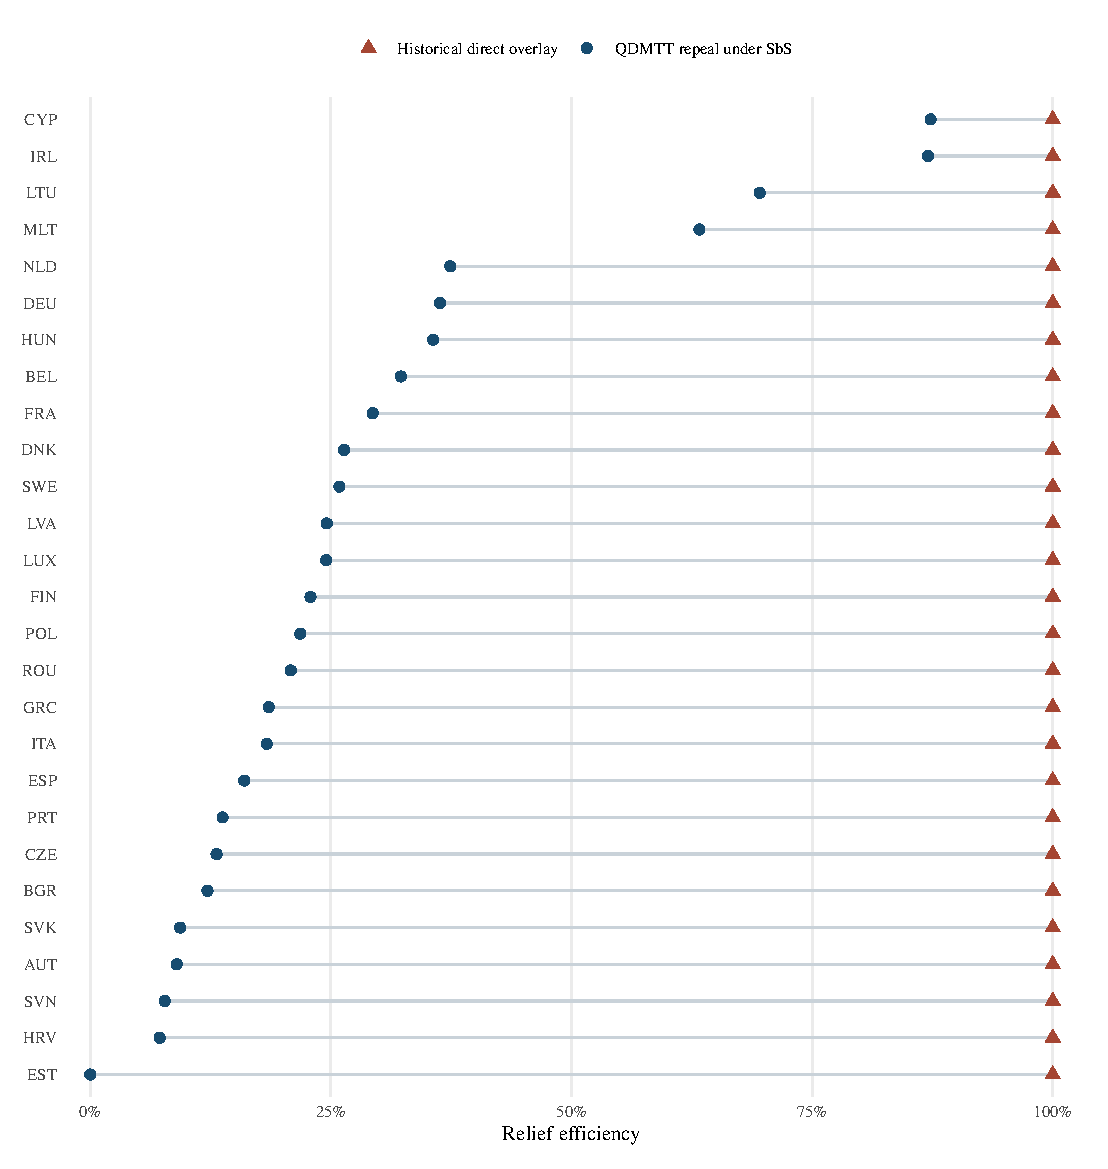
\includegraphics[width=\textwidth]{generated/paper_v2_figures/fig_v2_qdmtt_deviation_efficiency_vs_sbti.pdf}
\caption{Tax relief per unit of top-up revenue forgone, by Member State. Circles show the tax-cut efficiency of unilateral QDMTT repeal under SbS; triangles show the efficiency of a capped SBTI overlay with the QDMTT kept in place. FY2023, L3, full EU27 adoption benchmark.}
\label{fig:v2_qdmtt_game}
\end{figure}

The alternative to repeal is to keep the QDMTT and grant qualifying incentives up to the SBTI cap introduced in January 2026, the instrument through which \citet{janeba2023} and \citet{schjelderup2024} expect tax competition to continue. Because qualifying incentives raise the covered taxes used in every collector's computation, no other government can claim what the host forgoes: the overlay reaches firms at 100\% efficiency with zero foreign leakage in all 27 states. It delivers \usd5.64 billion of relief in FY2023 under L3 and \usd16.52 billion over 2021–2023, and it exceeds the relief from repeal in 18 of 27 states in FY2023 under L3 (19 of 27 under strict L4 over 2021–2023).\footnote{The SBTI overlay is a capacity proxy built from sectoral payroll and carrying-value caps allocated to low-taxed profit. Its efficiency measures who receives the relief and excludes the fiscal cost of funding new qualifying incentives.} Repeal delivers more where US-parented profit is large relative to physical substance. In Ireland, FY2023 repeal gives firms \usd4.57 billion against \usd0.44 billion under the overlay, and Cyprus, Malta, Luxembourg, the Netherlands and Hungary show the same ordering; in Croatia, Denmark and Lithuania the two differ by less than \usd3 million. Section \ref{sec:conclusion} draws these results together into an answer for finance ministries and for the literature.

\section{Conclusion}\label{sec:conclusion}

This section answers the question posed at the outset, draws out what the answer means for those who forecast and legislate, and sets out what public data cannot settle.

\subsection{Answer and implications}\label{sec:answer}

Disagreement about how much the minimum tax will raise is mostly disagreement about the tax base, and only marginally about how firms behave. In the 64-scenario design, the aggregation of effective tax rates and the bridge from accounting profit to the minimum-tax base jointly explain 84.7–91.8\% of the variance in EU27 revenue over the 2017–2023 and 2019–2023 windows. Noise in the estimated parameters accounts for at most 1.71\% of total variance, and the spread across scenarios exceeds the 90\% parameter interval of the preferred scenario by factors of $\Lambda=6.93$ and $\Lambda=14.99$. The behavioural response, which absorbs most of the empirical effort in this field, moves the total by less than the choice of how to read a country-by-country table.

The finding places the existing estimates on one map. The jurisdiction averages of \citet{barake2022} and the distributional base of \citet{hugger2026} are two settings of the same switch, and the move between them is the largest single source of disagreement. \citet{hanlon2023} identified the gap between accounting and taxable profit as material; the bridge quantifies it and shows that it decides the outcome in the conduit hubs. \citet{boukal2026} score behaviour for one state, and once the same response is scored jointly with the ordinary tax it brings home, the large destination economies gain on balance. The dominance result of \citet{devereux2022} holds exactly under the original allocation and survives SbS for a government that maximises revenue, while the capped incentives that \citet{janeba2023} and \citet{schjelderup2024} analyse become the cheaper route to relief in most Member States.

Three implications follow for finance ministries and revenue forecasters. First, they should settle how effective tax rates are measured within countries and how CbCR profit maps into the minimum-tax base, including the dividend purge, loss netting within subgroups, loss carryforwards and the unwinding of conduit structures in older vintages, before debating behavioural semi-elasticities; Section \ref{sec:decomposition} shows that these choices move the forecast by multiples. Second, behavioural responses should be scored together with the ordinary CIT that relocated profit pays at its destination, since the net effect has opposite signs in hubs and in large economies. Third, adopting a QDMTT remains the revenue-maximising choice under SbS, yet competition for real investment and for groups parented outside the United States moves to capped substance-based incentives, which deliver relief without leakage, while hubs dominated by US-parented groups face a repeal option that passes most of the forgone revenue to firms. These conclusions rest on public aggregates, which sets clear limits.

\subsection{Limitations and next steps}\label{sec:limitations}

Public aggregates cannot recover firm-level detail, so several results are bounds and should be read as such. Five limits matter. The public CbCR tables do not cross-classify subgroup ETRs by firm-level profit weights or ownership chains, so the distributional measure approximates the true distribution at host level. The accounting bridge approximates firm-level elections, deferred tax adjustments and loss carryforwards on bilateral cell aggregates. National budget benchmarks differ from the model in cash timing, fiscal windows and the take-up of safe harbours, so the back-test diagnoses where gaps arise and does not score point forecasts. Eligibility to collect under the UTPR is proxied by qualified IIR status in the Central Record of 1 May 2026, which overstates collectors wherever a UTPR has yet to qualify. Finally, three non-EU host-years in 2023 lack low-bracket tax accrued in pooled Table IV; Appendix \ref{app:measurement} shows that they move EU27 liability by less than 0.6\%.

Each limit has a remedy as new data arrive. The GloBE Information Returns that groups file from mid-2026 record the elections, covered taxes and loss positions that the bridge approximates, and research access to them under confidentiality would turn the bounds into point estimates. Administrative receipts for 2024 onwards will show how far the accounting adjustments and safe harbours close the gap to national budgets. The adoption record after 2026 offers a natural experiment for the repeal game: if hubs dominated by US-parented groups weaken their domestic top-up taxes while real-economy states turn to capped incentives, the pattern in Table \ref{tab:tab_v2_main_table8_qdmtt_repeal_game} will have anticipated it.

\bibliographystyle{apalike}
\bibliography{paper_v2_refs}

\clearpage
\appendix
\section{Data, profit reconciliation and notation}\label{app:data}
\draftstub{Pass 5}

\section{Measuring low-taxed profit, substance and the tax base}\label{app:measurement}
\draftstub{Pass 5}

\section{Behavioural estimation}\label{app:behaviour}
\draftstub{Pass 5}

\section{Factorial decomposition, uncertainty and country results}\label{app:decomposition}
\draftstub{Pass 5}

\section{Allocation law, the repeal game and replication}\label{app:allocation}
\draftstub{Pass 5}

\end{document}
